\documentclass[11pt,a4paper]{article}
\usepackage[utf8]{inputenc}
\usepackage[T1]{fontenc}
\usepackage[sc]{mathpazo}
\usepackage[scaled=0.92]{helvet}
\usepackage{microtype}
\usepackage[a4paper,top=2.6cm,bottom=2.4cm,left=2.4cm,right=2.4cm,headheight=14pt]{geometry}
\usepackage[table]{xcolor}
\usepackage{booktabs,array,enumitem,multirow}
\usepackage{tikz}
\usetikzlibrary{calc,positioning}
\usepackage{pgfplots}
\pgfplotsset{compat=1.16}
\usepackage[most]{tcolorbox}
\usepackage{titlesec}
\usepackage{needspace,etoolbox}
\usepackage{fancyhdr}
\usepackage{caption}
\usepackage{url}
\def\UrlBreaks{\do\/\do\-\do\_\do\.\do\=\do\?\do\&\do\a\do\b\do\c\do\d\do\e\do\f\do\g\do\h\do\i\do\j\do\k\do\l\do\m\do\n\do\o\do\p\do\q\do\r\do\s\do\t\do\u\do\v\do\w\do\x\do\y\do\z}
\Urlmuskip=0mu plus 1mu
\urlstyle{same}
\usepackage[hidelinks]{hyperref}

% ---- Palet (selaras dengan halaman dokumen pelengkap) ----
\definecolor{teal}{HTML}{0A6C6E}
\definecolor{tealdark}{HTML}{07484A}
\definecolor{ink}{HTML}{13262A}
\definecolor{muted}{HTML}{51666A}
\definecolor{rule}{HTML}{D3DEDC}
\definecolor{pale}{HTML}{EEF5F4}
\definecolor{amber}{HTML}{B7791F}
\definecolor{amberpale}{HTML}{FBF4E4}
\definecolor{well}{HTML}{CFE3E0}

\renewcommand{\tablename}{Tabel}
\renewcommand{\figurename}{Gambar}
\renewcommand{\refname}{Daftar Pustaka}
\color{ink}
\setlength{\parindent}{0pt}
\setlength{\parskip}{6.5pt plus 1pt}
\linespread{1.06}
\tolerance=1200
\emergencystretch=3em
\hyphenpenalty=1500
\setlist{itemsep=2.5pt,topsep=3pt,parsep=0pt,leftmargin=1.4em}
\setlist[itemize]{label={\color{teal}\textbullet}}
\renewcommand{\arraystretch}{1.22}
\setlength{\tabcolsep}{5pt}
\captionsetup{font={small,sf,color=muted},labelfont={bf,color=teal},labelsep=period,justification=raggedright,singlelinecheck=false,skip=5pt}

% ---- Judul bagian ----
\titleformat{\section}{\sffamily\bfseries\Large\color{ink}}{\color{teal}\thesection}{0.7em}{}[{\color{rule}\titlerule[0.6pt]}]
\titlespacing*{\section}{0pt}{18pt}{9pt}
\titleformat{\subsection}{\sffamily\bfseries\normalsize\color{tealdark}}{\color{teal}\thesubsection}{0.6em}{}
\titlespacing*{\subsection}{0pt}{11pt}{3pt}

% ---- Kepala dan kaki halaman ----
\pagestyle{fancy}
\fancyhf{}
\renewcommand{\headrulewidth}{0pt}
\fancyhead[L]{\sffamily\scriptsize\color{muted}\textsc{Alergen}\ \raisebox{0.15ex}{\tiny$\bullet$}\ Alergen Reader, Dokumentasi Teknis}
\fancyhead[R]{\sffamily\scriptsize\color{muted}Kit Diagnostik Alergi Berbasis Patch}
\fancyfoot[L]{\sffamily\scriptsize\color{muted}Universitas Airlangga \ $\cdot$ \ IDS000011522}
\fancyfoot[R]{\sffamily\small\bfseries\color{teal}\thepage}
\renewcommand{\headrule}{\color{rule}\hrule width\headwidth height 0.5pt}
\renewcommand{\headrulewidth}{0.5pt}
\fancypagestyle{plain}{\fancyhf{}\renewcommand{\headrulewidth}{0pt}\fancyfoot[R]{\sffamily\small\bfseries\color{teal}\thepage}}

% ---- Tabel ----
\newcommand{\tH}[1]{\textcolor{white}{\sffamily\bfseries\small #1}}
\newcommand{\tabstart}{\small\rowcolors{2}{white}{pale}\arrayrulecolor{rule}}
\newcommand{\hdrrow}{\rowcolor{tealdark}}
\newcolumntype{L}[1]{>{\raggedright\arraybackslash}p{#1}}
\newcolumntype{R}[1]{>{\raggedleft\arraybackslash}p{#1}}
\setlength{\aboverulesep}{0pt}\setlength{\belowrulesep}{0pt}
\renewcommand{\toprule}{\arrayrulecolor{tealdark}\specialrule{0.9pt}{0pt}{0pt}\arrayrulecolor{rule}}
\renewcommand{\bottomrule}{\arrayrulecolor{tealdark}\specialrule{0.9pt}{0pt}{0pt}\arrayrulecolor{rule}}

% ---- Kotak catatan dan kartu angka ----
\newtcolorbox{catatan}[1][Catatan]{enhanced,breakable,colback=amberpale,colframe=amberpale,boxrule=0pt,
  borderline west={2.2pt}{0pt}{amber},arc=1.5pt,left=10pt,right=8pt,top=6pt,bottom=6pt,
  before skip=8pt,after skip=10pt,
  title={\sffamily\bfseries\small\color{amber}\MakeUppercase{#1}},coltitle=amber,
  attach boxed title to top left={yshift=-2mm,xshift=0pt},boxed title style={empty,left=0pt,top=0pt,bottom=0pt},
  fonttitle=\sffamily,coltext=ink,before upper={\vspace{2pt}}}
\newtcolorbox{kartu}[2]{enhanced,colback=pale,colframe=pale,boxrule=0pt,arc=3pt,
  left=8pt,right=6pt,top=6pt,bottom=6pt,halign=left,
  borderline west={2.5pt}{0pt}{teal},
  before upper={{\sffamily\bfseries\LARGE\color{teal}#1}\par\vspace{1pt}},
  fontupper=\sffamily\scriptsize\color{muted},height=1.95cm,valign=top}
\newcommand{\kartuRow}[4]{%
 \begin{tcbraster}[raster columns=#1,raster equal height,raster column skip=7pt,raster row skip=7pt]#2#3#4\end{tcbraster}\vspace{9pt}}

% ---- Sampul ----
\newcommand{\patchmotif}[2]{% #1 skala, #2 warna garis
 \begin{scope}[scale=#1]
 \draw[#2,line width=1.2pt,rounded corners=9pt] (0,0) rectangle (15,6);
 \foreach \r in {0,1}{\foreach \c in {0,...,4}{
   \draw[#2,line width=1pt] ({1.9+\c*2.7},{4.1-\r*2.2}) circle (0.9);}}
 \end{scope}}

\newcommand{\makecover}[5]{% kode, judul, subjudul, tagline, ringkasan satu kalimat
\begin{titlepage}
\thispagestyle{empty}
\begin{tikzpicture}[remember picture,overlay]
 \fill[tealdark] (current page.north west) rectangle ($(current page.north east)+(0,-17.2cm)$);
 \fill[teal!85!tealdark] ($(current page.north east)+(0,-17.2cm)$) -- ($(current page.north east)+(-10cm,-17.2cm)$) -- ($(current page.north east)+(0,-10.8cm)$) -- cycle;
 \begin{scope}[shift={($(current page.north east)+(-9.9cm,-6.4cm)$)}]
   \patchmotif{0.5}{white!35}
 \end{scope}
 \node[anchor=north west,text=white!70,font=\sffamily\small\bfseries,align=left] at ($(current page.north west)+(2.4cm,-2.7cm)$) {\textsc{Alergen \ $\cdot$ \ Universitas Airlangga}};
 \node[anchor=north west,text=white,font=\sffamily\bfseries\fontsize{44}{44}\selectfont] at ($(current page.north west)+(2.4cm,-7.4cm)$) {#1};
 \node[anchor=north west,text=white,font=\sffamily\bfseries\fontsize{26}{31}\selectfont,text width=14.2cm,align=left] at ($(current page.north west)+(2.4cm,-10.2cm)$) {#2};
 \node[anchor=north west,text=white!85,font=\sffamily\fontsize{13}{17}\selectfont,text width=14cm,align=left] at ($(current page.north west)+(2.4cm,-14.1cm)$) {\hyphenpenalty=10000\exhyphenpenalty=10000 #3};
 \node[anchor=north west,text=ink,font=\fontsize{12}{17}\selectfont,text width=15.2cm,align=left] at ($(current page.north west)+(2.4cm,-18.8cm)$) {#4};
 \draw[teal,line width=2pt] ($(current page.north west)+(2.4cm,-21.9cm)$) -- ++(2.2cm,0);
 \node[anchor=north west,text=muted,font=\sffamily\small,text width=15cm,align=left] at ($(current page.north west)+(2.4cm,-22.4cm)$) {%
  \textbf{\color{ink}Kit Diagnostik Alergi Berbasis Patch (Alergen)}\\[3pt]
  Universitas Airlangga, Surabaya\\
  Paten Sederhana IDS000011522\\
  Oktober 2026};
 \node[anchor=south east,text=muted,font=\sffamily\scriptsize,align=right] at ($(current page.south east)+(-2.4cm,1.6cm)$) {#5};
\end{tikzpicture}
\end{titlepage}
\newpage}

\definecolor{sr1}{HTML}{8AA6AB}
\definecolor{sr2}{HTML}{3FA7A3}
\definecolor{sr3}{HTML}{0A6C6E}
\definecolor{sr4}{HTML}{B7791F}
\pgfplotsset{natbase/.style={width=0.95\linewidth,height=6.2cm,
  every axis label/.append style={font=\sffamily\scriptsize,color=muted},
  tick label style={font=\sffamily\scriptsize,color=muted},
  legend style={font=\sffamily\scriptsize,draw=rule,fill=white,at={(0.5,-0.2)},anchor=north},
  grid=major,grid style={color=rule,line width=0.4pt},
  axis line style={color=rule},tick style={color=rule},
  scaled ticks=false,/pgf/number format/.cd,1000 sep={.},fixed,precision=0,/tikz/.cd},
  natplot/.style={natbase,xtick={1,2,3,4,5},xticklabels={2028,2029,2030,2031,2032}}}
\hypersetup{pdftitle={Alergen Reader, Dokumentasi Teknis dan Panduan Desain},pdfauthor={Tim Alergen, Universitas Airlangga}}

\pretocmd{\section}{\Needspace{7\baselineskip}}{}{}
\pretocmd{\subsection}{\Needspace{4\baselineskip}}{}{}

\usepackage{graphicx,longtable,float,subcaption}
\graphicspath{{gambar/}}
\captionsetup[sub]{font={small,sf,color=muted},labelfont={bf,color=ink},skip=4pt}
\newcommand{\tcell}[1]{#1}
\setlength{\LTpre}{6pt}\setlength{\LTpost}{6pt}
\begin{document}

\makecover{Reader}{Alergen Reader}{Dokumentasi Teknis dan Panduan Desain}{Aplikasi seluler untuk membaca reaksi kulit pada patch Alergen: dokumentasi produk, arsitektur, pipeline analisis citra, sistem desain, aksesibilitas, pengujian, dan build. Tiga belas tangkapan layar dirender langsung dari kode sumber pada 390\,x\,844 piksel logis.}{Versi 0.2.0, Laboratorium LIHTR, Universitas Airlangga}

\renewcommand{\contentsname}{Daftar Isi}
\tableofcontents
\clearpage

\section*{Ringkasan}
\addcontentsline{toc}{section}{Ringkasan}

\kartuRow{4}
{\begin{kartu}{13}{}tangkapan layar nyata sebagai bukti visual\end{kartu}}
{\begin{kartu}{45}{}uji unit dan widget, semuanya lulus\end{kartu}}
{\begin{kartu}{10}{}sumur alergen dari satu foto, dibaca di perangkat\end{kartu}
\begin{kartu}{21,0 MB}{}APK arm64-v8a, build rilis per ABI\end{kartu}}

Pembacaan uji tempel (\textit{patch test}) kulit selama ini mengandalkan pengamatan
mata dan pencatatan manual, sehingga hasilnya bergantung pada penilai dan sulit
dibandingkan antarwaktu. Alergen Reader menjawab kesenjangan itu dengan cara yang
terbatas dan jujur: aplikasi mengambil satu foto rangka pembaca 20\,x\,50 mm yang
berisi sepuluh sumur alergen berdiameter 7 mm, mengoreksi perspektifnya, mengukur
kemerahan tiap sumur sebagai selisih warna CIELAB terhadap kulit sekitar, lalu
mengusulkan skor bergaya ICDRG. Aplikasi tidak mendiagnosis apa pun. Saran skor
bersifat usulan; timpaan, catatan morfologi, dan konfirmasi akhir tetap milik
tenaga kesehatan.

Yang dibangun pada versi 0.2.0 adalah aplikasi Flutter untuk Android (dan siap
iOS) dengan antarmuka dua peran: tenaga kesehatan yang menjalankan seluruh alur
pembacaan, dan pasien yang hanya memotret pada jadwal serta menerima peringatan
tanda bahaya. Seluruh pengolahan citra berjalan di perangkat tanpa jaringan.
Riwayat pembacaan tersimpan di SQLite lokal dengan kunci pasien berupa kode,
bukan nama, dan dapat diekspor sebagai CSV per sumur. Sebuah mode demo merakit
tiga foto kulit sintetis lalu menganalisisnya dengan pipeline yang sama dengan
foto nyata, sehingga pengguna baru dapat mencoba seluruh alur tanpa data pasien.

Bukti bahwa sistem berjalan bersifat dapat direproduksi. Sembilan belas berkas
uji otomatis berisi 45 uji unit dan widget lulus tanpa kecuali, mencakup pipeline
analisis pada foto sintetis, penilaian, ekspor CSV, timpaan dokter, penyembunyian
skor pada peran pasien, dan render enam layar utama pada 360\,x\,640 dengan skala
teks 1,3 tanpa \textit{overflow}. Harness \texttt{tool/screenshots\_test.dart}
merender tiga belas tangkapan layar pada 390\,x\,844 dengan font terbundel dan
foto demo yang dianalisis pipeline sungguhan; ke-13 berkas itulah yang menjadi
bukti visual dokumen ini. Build rilis APK terpisah per ABI sukses dengan ukuran
18,9 MB (armeabi-v7a), 21,0 MB (arm64-v8a), dan 22,5 MB (x86\_64).

\begin{catatan}[Batasan utama]
Ambang skor 2,5 / 5 / 10 pada $\Delta a^*$ beserta faktor warna kulit Fitzpatrick adalah titik awal dari uji sintetis yang belum divalidasi klinis. Jadwal pembacaan definitif belum ditetapkan, dan aspek privasi lanjutan seperti enkripsi penyimpanan masih menjadi pekerjaan berikutnya. Bagian 8 merinci daftar itu beserta rencana validasinya.
\end{catatan}

% ============================ BAB 1 ============================
\section{Pendahuluan}

\subsection{Latar belakang}

Uji tempel alergen adalah pemeriksaan yang menempelkan ekstrak alergen pada kulit
punggung pasien selama beberapa jam, lalu membaca reaksi yang muncul. Pembacaan
yang bermakna terjadi pada 48 sampai 96 jam setelah pemasangan, dan keputusan
klinisnya bergantung pada seberapa merah dan tebal reaksi tiap alergen. Cara
membaca yang lazim, yaitu mengamati dan mencatat manual, memiliki dua masalah
praktis: hasil antarpenilai bisa berbeda, dan perbandingan antarwaktu pada orang
yang sama sulit dijaga konsisten karena tidak ada pengukuran yang tersimpan.

Alergen Reader membangun satu bagian kecil dari rantai itu: pengukuran. Dengan
satu foto tegak dari rangka pembaca yang posisi sumurnya tetap, aplikasi
menghasilkan tiga besaran per sumur, yaitu $\Delta a^*$ (pergeseran kemerahan),
$\Delta L^*$ (pergeseran kecerahan), dan fraksi piksel merah, semuanya relatif
terhadap kulit sekitar rangka pada foto yang sama. Karena pembandingnya diambil
dari foto itu sendiri, variasi pencahayaan dan warna kulit dasar ikut ternormalkan.

\subsection{Ruang lingkup}

Dokumen ini menjelaskan produk, arsitektur, sistem desain antarmuka, pengujian,
dan cara membangun aplikasi pada versi 0.2.0. Pembahasan kode merujuk pada berkas
nyata di repositori; setiap angka yang muncul dapat dilacak ke berkas, uji, atau
perintah build yang disebutkan. Tiga belas tangkapan layar pada Bagian 4 dan Bagian 5
dirender oleh harness uji, bukan dirangkai manual, sehingga merupakan kondisi
aplikasi sesungguhnya.

\subsection{Batasan medis}

Aplikasi ini adalah alat bantu dokumentasi dan pengukuran, bukan alat diagnosis.
Tiga pengaman tertanam di kode dan diuji otomatis. Pertama, saran skor dari foto
hanya mengukur eritema; morfologi seperti infiltrasi, papul, vesikel, dan bula
tidak dapat dinilai dari foto dan wajib dicentang tenaga kesehatan, yang hanya
dapat menaikkan saran, tidak pernah menurunkannya. Kedua, tenaga kesehatan selalu
dapat menimpa skor, termasuk kode IR untuk reaksi iritan, dan pembacaan baru
berstatus final setelah tombol Konfirmasi ditekan. Ketiga, peran pasien secara
bawaan tidak melihat skor sama sekali; yang tampil hanyalah konfirmasi foto
tersimpan beserta tanda bahaya yang wajib segera ke dokter.

Ambang penilaian pada Tabel~\ref{tab:ambang} adalah titik awal dari uji sintetis
dan belum divalidasi pada pasien. Sebelum dipakai klinis, kalibrasi terhadap
penilaian dua dokter kulit independen wajib dilakukan sebagaimana dirinci pada
Bagian 8.

\subsection{Pembaca yang dituju}

Dokumen ini ditujukan bagi pengembang yang akan melanjutkan kode, desainer yang
akan memelihara sistem desain Clinical Ink, dan tenaga kesehatan serta peneliti
yang perlu memahami apa yang diukur aplikasi beserta batasnya. Pembaca diasumsikan
familiar dengan dasar pemrograman seluler; istilah domain dan teknis dijelaskan
pada Lampiran B.

% ============================ BAB 2 ============================
\section{Gambaran Produk}

\subsection{Alur pengguna dari ujung ke ujung}

Alur tenaga kesehatan berjalan sebagai berikut. Dari Beranda, tombol Pembacaan
baru membuka layar kamera dengan panduan rangka. Foto yang diambil dipraproses
(rotasi EXIF, penurunan resolusi maksimal 2000 piksel pada sisi panjang), lalu
layar sudut menampilkan usulan empat sudut rangka hasil deteksi otomatis untuk
dikonfirmasi atau digeser. Setelah kode pasien, jam pembacaan, dan tipe kulit
Fitzpatrick diisi, aplikasi menjalankan analisis dan menampilkan layar hasil:
foto terkoreksi dengan cincin warna skor per sumur, metrik ringkas, daftar sepuluh
sumur dengan saran otomatis, serta kontrol timpaan dan morfologi. Konfirmasi
menandai pembacaan final; riwayat menyimpan semuanya dan dapat diekspor CSV.

Alur pasien lebih pendek dan sengaja dibuat tumpul informasi: buka aplikasi pada
jadwal, foto terpandu dengan peringatan bahasa awam bila foto buram atau gelap,
lalu layar hasil hanya menyatakan foto tersimpan dan menampilkan tanda bahaya.
Skor tidak muncul kecuali klinik mengaktifkan sakelar skor sementara pada
Pengaturan.

\subsection{Sepuluh alergen resmi}

Urutan sumur pada rangka mengikuti daftar resmi dari sumber
alergen.airlangga.link yang tersimpan di \texttt{assets/config/allergens.json}:
tungau debu rumah, udang, susu sapi, daging, ayam, telur, gandum, kacang tanah,
kelapa atau santan, serta serbuk sari atau polen. Nomor sumur di seluruh
antarmuka dan CSV merujuk urutan ini, sehingga pembacaan antarwaktu dan
antarperangkat dapat diperbandingkan tanpa ambigu.

\subsection{Mode demo: data sintetis melalui pipeline nyata}

Mode demo pada Pengaturan merakit tiga foto kulit sintetis (DEMO-01 pada 48 jam,
DEMO-02 pada 72 jam, DEMO-03 pada 96 jam, semuanya Fitzpatrick IV) lengkap dengan
rangka putih dan sepuluh sumur yang kemerahannya bertingkat, menyimpannya sebagai
berkas gambar, lalu menganalisisnya dengan fungsi analisis yang sama dengan foto
kamera. Artinya, angka yang tampil di layar hasil demo adalah keluaran pipeline
sungguhan, bukan angka karangan; uji \texttt{demo\_seed\_test.dart} memverifikasi
tiga sesi berisi 30 sumur dengan skor yang benar-benar bervariasi, timpaan dan
morfologi demo, serta CSV 31 baris. Data demo selalu bertanda DEMO dan tidak
pernah bercampur dengan data pasien nyata; uji juga mengunci bahwa menghapus
data demo tidak menghapus sesi nyata.

\subsection{Penyimpanan riwayat}

Riwayat tersimpan di SQLite perangkat melalui sqflite, satu baris per pembacaan
beserta foto terkoreksi dan metrik per sumur dalam format JSON yang lolos uji
bolak-balik (\textit{round trip}). Kunci pasien berupa kode, bukan nama. Tidak
ada unggahan jaringan pada versi ini; ekspor CSV berbagi satu berkas berisi
seluruh pembacaan, satu baris per sumur, melalui mekanisme berbagi sistem.

% ============================ BAB 3 ============================
\section{Arsitektur dan Pipeline}

\subsection{Peta folder}

\begin{table}[H]
\centering
\caption{Struktur folder utama dan isinya.}
\label{tab:folder}
\tabstart
\begin{tabular}{@{}L{4.6cm}L{9.6cm}@{}}
\toprule
\hdrrow\tH{Folder} & \tH{Isi} \\
\midrule
\tcell{lib/core} & Pipeline murni: praproses foto, deteksi rangka, homografi,
CIELAB, analisis, penilaian. Tanpa dependensi Flutter sehingga mudah diuji. \\
\tcell{lib/data} & Penyimpanan SQLite sesi, settings JSON, ekspor CSV, perakit
data demo. \\
\tcell{lib/models} & Tipe domain WellReading dan ReadingSession beserta
serialisasi JSON. \\
\tcell{lib/screens} & Delapan layar: onboarding, kerangka tab, beranda, kamera,
sudut, hasil, riwayat, pengaturan. \\
\tcell{lib/state} & AppState: peran, konfigurasi, sakelar pasien, sesi, data
demo, flag onboarding. \\
\tcell{lib/theme, lib/widgets} & Token desain Clinical Ink dan komponen bersama
(kartu, tombol, chip skor, MetricStrip, banner, header, LegendSheet). \\
\tcell{test} & 45 uji unit dan widget pada sembilan berkas. \\
\tcell{tool} & Harness screenshot yang merender bukti visual ke shots/. \\
\tcell{assets/config} & Geometri rangka dan nama alergen; dapat diubah tanpa
kompilasi ulang. \\
\bottomrule
\end{tabular}
\end{table}

Arsitektur mengikuti arah dependensi satu jalur: layar membaca state, state
memanggil data dan domain, dan \texttt{lib/core} tidak mengenal Flutter sama
sekali. Selama redesain antarmuka pada 0.2.0, lapisan core sengaja tidak
disentuh logikanya; satu-satunya perubahan lapisan data adalah penambahan flag
\texttt{onboardingDone} pada settings.

\subsection{Pipeline analisis citra}

Pipeline berjalan sepenuhnya di perangkat dan terdiri atas enam tahap berikut.

\begin{enumerate}
\item \textbf{Persiapan foto.} Dekode JPEG, rotasi sesuai EXIF, penurunan
resolusi hingga maksimal 2000 piksel pada sisi panjang, lalu simpan kembali
sebagai JPEG bersih.
\item \textbf{Deteksi rangka.} Rangka putih dibedakan dari kulit lewat
saturasi rendah (di bawah 0,137) dengan kecerahan tinggi (di atas 0,725).
Komponen terbesar diambil, empat titik ekstremnya dicari, lalu didorong keluar
4\% untuk mengompensasi sudut rangka yang membulat. Hasil selalu ditampilkan di
layar sudut untuk dikonfirmasi atau digeser manual; deteksi hanyalah usulan.
\item \textbf{Rektifikasi.} Homografi empat titik memetakan foto ke kanvas
10 piksel per mm dengan margin 10 mm. Seluruh geometri berikutnya memakai
milimeter, sehingga posisi sumur selalu sama di setiap pembacaan.
\item \textbf{Warna kulit acuan.} Cincin kulit 2 sampai 8 mm di luar rangka
diambil, piksel dengan L* di luar persentil 10 sampai 90 dibuang, lalu dihitung
median L*a*b*. Median inilah pembanding tiap sumur sekaligus penormalkan
pencahayaan.
\item \textbf{Metrik per sumur.} Pada 80\% jari-jari sumur (menghindari bayangan
tepi rangka) dihitung $\Delta a^*$ rerata terpangkas persentil 10 sampai 90,
$\Delta L^*$, dan fraksi piksel dengan $\Delta a^*>3$.
\item \textbf{Saran skor dan kualitas.} $\Delta a^*$ dipetakan ke simbol ICDRG
menurut Tabel~\ref{tab:ambang}, lalu hanya dapat dinaikkan oleh morfologi yang
dicentang dokter. Pemeriksaan kualitas (ketajaman varians Laplacian pada cincin
kulit, jumlah piksel kulit, kegelapan, pantulan, kemiringan perspektif, dan
resolusi) menghasilkan peringatan berbahasa awam bila foto kurang layak dibaca.
\end{enumerate}

\begin{table}[H]
\centering
\caption{Pemetaan usulan skor dari $\Delta a^*$ sebelum faktor Fitzpatrick.
Ambang adalah titik awal uji sintetis, belum tervalidasi klinis.}
\label{tab:ambang}
\tabstart
\begin{tabular}{@{}L{3.4cm}L{2.6cm}L{8.2cm}@{}}
\toprule
\hdrrow\tH{$\Delta a^*$} & \tH{Saran foto} & \tH{Arti ICDRG} \\
\midrule
\tcell{$<2{,}5$} & \tcell{$-$} & \tcell{Negatif} \\
\tcell{$2{,}5$ sampai $<5$} & \tcell{$?+$} & \tcell{Meragukan, eritema samar} \\
\tcell{$5$ sampai $<10$} & \tcell{$+$} & \tcell{Positif lemah: eritema, mungkin infiltrasi} \\
\tcell{$\geq 10$} & \tcell{$++$} & \tcell{Positif kuat} \\
\bottomrule
\end{tabular}
\end{table}

Faktor warna kulit Fitzpatrick (1,0 untuk I sampai III; 0,85 untuk IV; 0,7 untuk
V dan VI) menurunkan ambang pada kulit lebih gelap karena eritema lebih sulit
terbaca lewat kanal a*. Contohnya pada Fitzpatrick IV, ambang 2,5 menjadi 2,1;
rentang inilah yang ditampilkan pada sheet Panduan simbol skor (Gambar~\ref{fig:legend}).

\subsection{Offline pertama dan format penyimpanan}

Tidak ada panggilan jaringan pada versi ini. Foto asli dan hasil analisis
tersimpan di penyimpanan aplikasi, metrik per sumur diserialisasi sebagai JSON
pada kolom sesi, dan pengaturan klinik pada berkas JSON terpisah sehingga satu
penulisan tidak menghapus kunci lainnya. Konfigurasi geometri dan nama alergen
dimuat dari aset saat mulai; bila berkas rusak, aplikasi jatuh ke nilai bawaan
dan menampilkan indikator halus di Pengaturan, sebuah perilaku yang diuji pada
\texttt{config\_test.dart}.

\subsection{Dependensi dan alasannya}

\begin{table}[H]
\centering
\caption{Dependensi publik beserta alasan pemakaiannya.}
\label{tab:dependensi}
\tabstart
\begin{tabular}{@{}L{3.2cm}L{11.0cm}@{}}
\toprule
\hdrrow\tH{Paket} & \tH{Alasan} \\
\midrule
\tcell{provider} & State management ringan; AppState sebagai ChangeNotifier
cukup untuk skala aplikasi. \\
\tcell{intl} & Format tanggal dan angka lokal id (koma desimal, nama bulan). \\
\tcell{sqflite} & Penyimpanan riwayat terstruktur di perangkat. \\
\tcell{path\_provider} & Lokasi direktori foto dan berkas sementara. \\
\tcell{camera, image\_picker} & Pengambilan foto dengan panduan rangka dan
fallback galeri. \\
\tcell{image} & Dekode, enkode, dan manipulasi piksel seluruh pipeline. \\
\tcell{share\_plus} & Berbagi CSV ekspor melalui mekanisme sistem. \\
\tcell{flutter\_lints} & Aturan analisis statis (dev). \\
\bottomrule
\end{tabular}
\end{table}

Tidak ada dependensi baru selama redesain 0.2.0; kebutuhan antarmuka diselesaikan
dengan widget dan painter internal agar payload dan permukaan audit tetap kecil.

% ============================ BAB 4 ============================
\section{Sistem Desain Clinical Ink}

\subsection{Filosofi}

Clinical Ink memilih bahasa visual klinik yang tenang: permukaan putih bersih di
atas kanvas hangat, garis rambut 1 px menggantikan bayangan, satu aksen pinus
untuk afordansi, dan tinta hampir hitam untuk teks. Judul display memakai
Instrument Serif sementara seluruh teks dan angka memakai Inter dengan angka
tabular agar kolom metrik sejajar. Gerak standar 220 ms dengan kurva
easeOutCubic, dan hormat pada pengaturan animasi sistem. Filosofinya sederhana:
warna hanya untuk makna (skor, bahaya, status), bukan hiasan, sehingga keputusan
klinis yang ditampilkan tidak bersaing dengan dekorasi.

\begin{table}[H]
\centering
\caption{Token warna inti dan fungsinya.}
\label{tab:warna}
\tabstart
\begin{tabular}{@{}L{3.4cm}L{2.2cm}L{8.6cm}@{}}
\toprule
\hdrrow\tH{Token} & \tH{Hex} & \tH{Fungsi} \\
\midrule
\tcell{canvas} & \tcell{\#F6F5F2} & \tcell{Latar layar, hangat, bukan putih steril.} \\
\tcell{surface} & \tcell{\#FFFFFF} & \tcell{Kartu dan lembar konten.} \\
\tcell{ink / inkSoft} & \tcell{\#0E1113 / \#22282D} & \tcell{Teks utama dan isi kartu gelap (hero).} \\
\tcell{slate / mist} & \tcell{\#5C6670 / \#8A939C} & \tcell{Keterangan dan ikon nonaktif.} \\
\tcell{hairline / hairlineStrong} & \tcell{\#E6E3DC / \#D5D1C8} & \tcell{Pemisah dan garis rambut pengganti bayangan.} \\
\tcell{accent / accentSoft} & \tcell{\#1D5C52 / \#EAF0EE} & \tcell{Aksen tindakan dan isian info lembut.} \\
\tcell{danger / dangerSoft} & \tcell{\#A02A22 / \#F7ECEA} & \tcell{Tanda bahaya dan isian peringatan keras.} \\
\tcell{onInk} & \tcell{\#F4F2ED} & \tcell{Teks di atas isian tinta.} \\
\tcell{cornerHandle} & \tcell{\#FF5252} & \tcell{Handle sudut rangka di layar koreksi.} \\
\bottomrule
\end{tabular}
\end{table}

Skor memakai tujuh warna bergradasi dari hijau tua (negatif) ke merah tua (sangat
kuat), ditambah ungu untuk reaksi iritan dan kelabu untuk sumur tak teruji. Warna
tidak pernah menjadi satu-satunya pembawa makna: setiap simbol selalu disertai
label dan urutan dapat dibaca lewat sheet legenda.

\begin{table}[H]
\centering
\caption{Tipografi: dua keluarga, peran terpisah.}
\label{tab:tipografi}
\tabstart
\begin{tabular}{@{}L{3.9cm}L{2.5cm}L{2.2cm}L{5.8cm}@{}}
\toprule
\hdrrow\tH{Gaya} & \tH{Keluarga} & \tH{Ukuran} & \tH{Pemakaian} \\
\midrule
\tcell{display XL, L, M} & \tcell{Instrument Serif} &
\tcell{40, 32, 26} & \tcell{Judul layar; maksimal satu gaya display per layar.} \\
\tcell{titleXL, titleL, titleM} & \tcell{Inter 600} &
\tcell{22/28, 18/24, 16/22} & \tcell{Judul bagian dan baris daftar.} \\
\tcell{body, bodyStrong} & \tcell{Inter 400/600} & \tcell{15/22} &
\tcell{Teks paragraf.} \\
\tcell{label} & \tcell{Inter 600} & \tcell{12/16} & \tcell{Label kapital dengan
jarak huruf; eyebrow dan seksi.} \\
\tcell{caption} & \tcell{Inter 400} & \tcell{12,5/18} & \tcell{Keterangan dan
catatan kaki layar.} \\
\tcell{metric} & \tcell{Inter 600 tabular} & \tcell{15/20} & \tcell{Angka metrik;
angka tabular agar kolom sejajar.} \\
\bottomrule
\end{tabular}
\end{table}

Komponen bersama yang dibangun di atas token itu antara lain SurfaceCard dan
InkCard (radius 22), tombol tiga tingkat (utama 54 px, sekunder garis rambut,
senyap teks), GradeChip berbentuk pil, MetricStrip tiga kolom dengan pemisah
vertikal, banner tiga varian dengan garis aksen 3 px, ScreenHeader, SectionLabel,
SettingRow, EmptyState, serta AppShell tiga tab dengan bilah navigasi kustom
yang menandai tab aktif lewat garis aksen 3\,x\,16 px.

\subsection{Onboarding}

Tiga halaman pengantar tampil sekali sebelum pengguna masuk aplikasi, lalu dapat
dibuka ulang dari Pengaturan. Halaman-halaman itu menjawab tiga pertanyaan
pengguna baru: apa yang dibaca aplikasi (reaksi sepuluh sumur dari satu foto),
bagaimana cara memotretnya (tegak dan ukuran tetap lewat koreksi sudut), dan di
mana posisi aplikasi dalam keputusan klinis (skor adalah usulan, keputusan tetap
milik tenaga kesehatan). Latar tinta penuh dengan ilustrasi garis memisahkan
pengantar dari isi aplikasi yang terang, sekaligus menjadi satu-satunya tempat
gradien radial lembut dipakai.

\begin{figure}[!htbp]
\centering
\begin{minipage}[t]{0.30\textwidth}
\centering
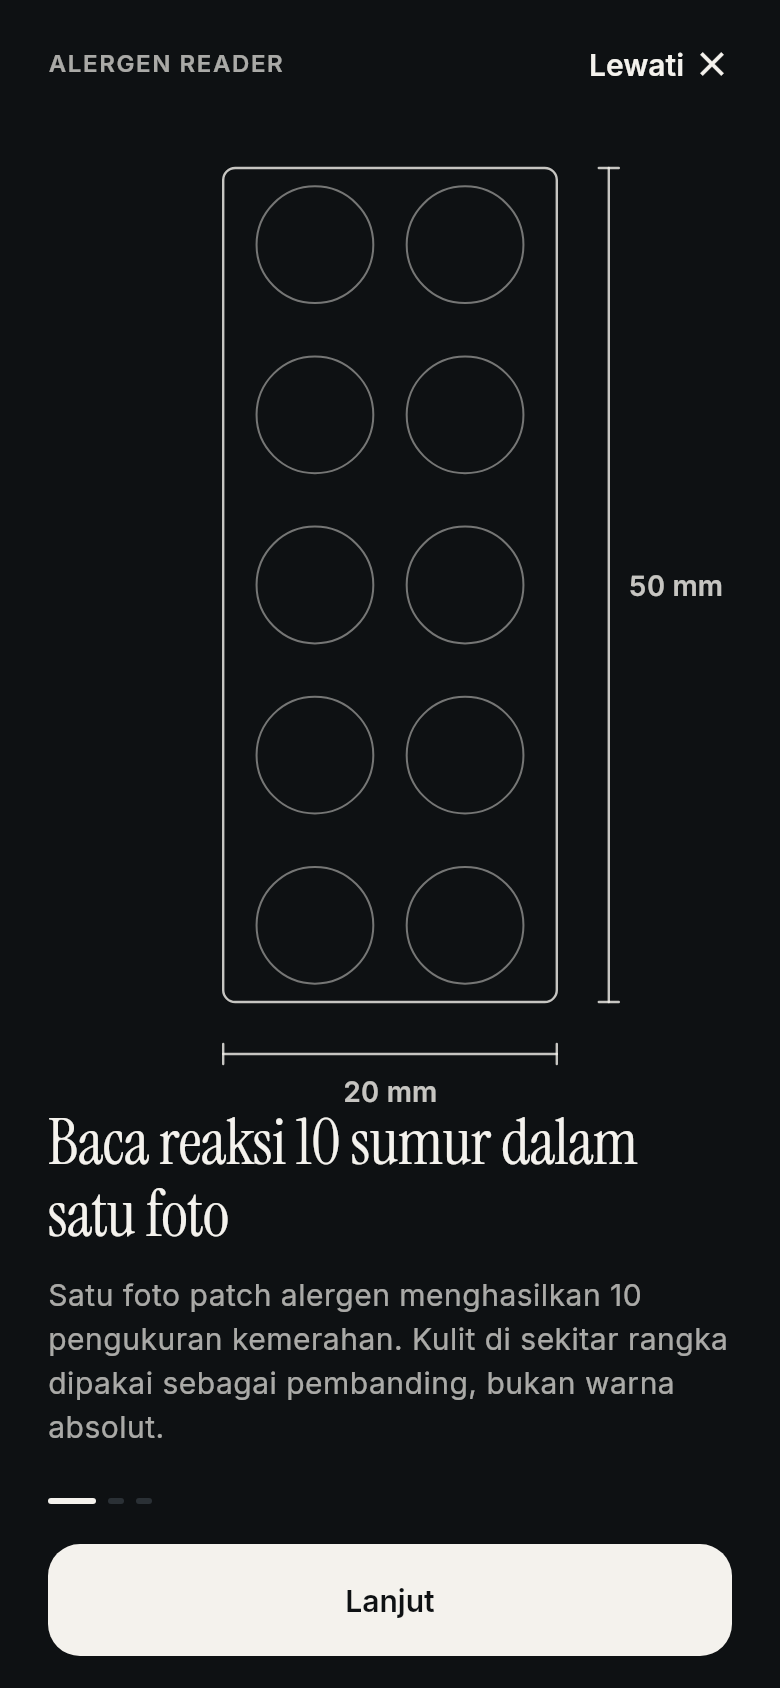
\includegraphics[width=\linewidth]{01_onboarding_1.png}
\subcaption{Halaman 1: rangka 2\,x\,5 dengan sepuluh sumur dan garis ukur 20 serta
50 mm menyampaikan bahwa satu foto menghasilkan sepuluh pengukuran.}\label{fig:onb1}
\end{minipage}\hfill
\begin{minipage}[t]{0.30\textwidth}
\centering
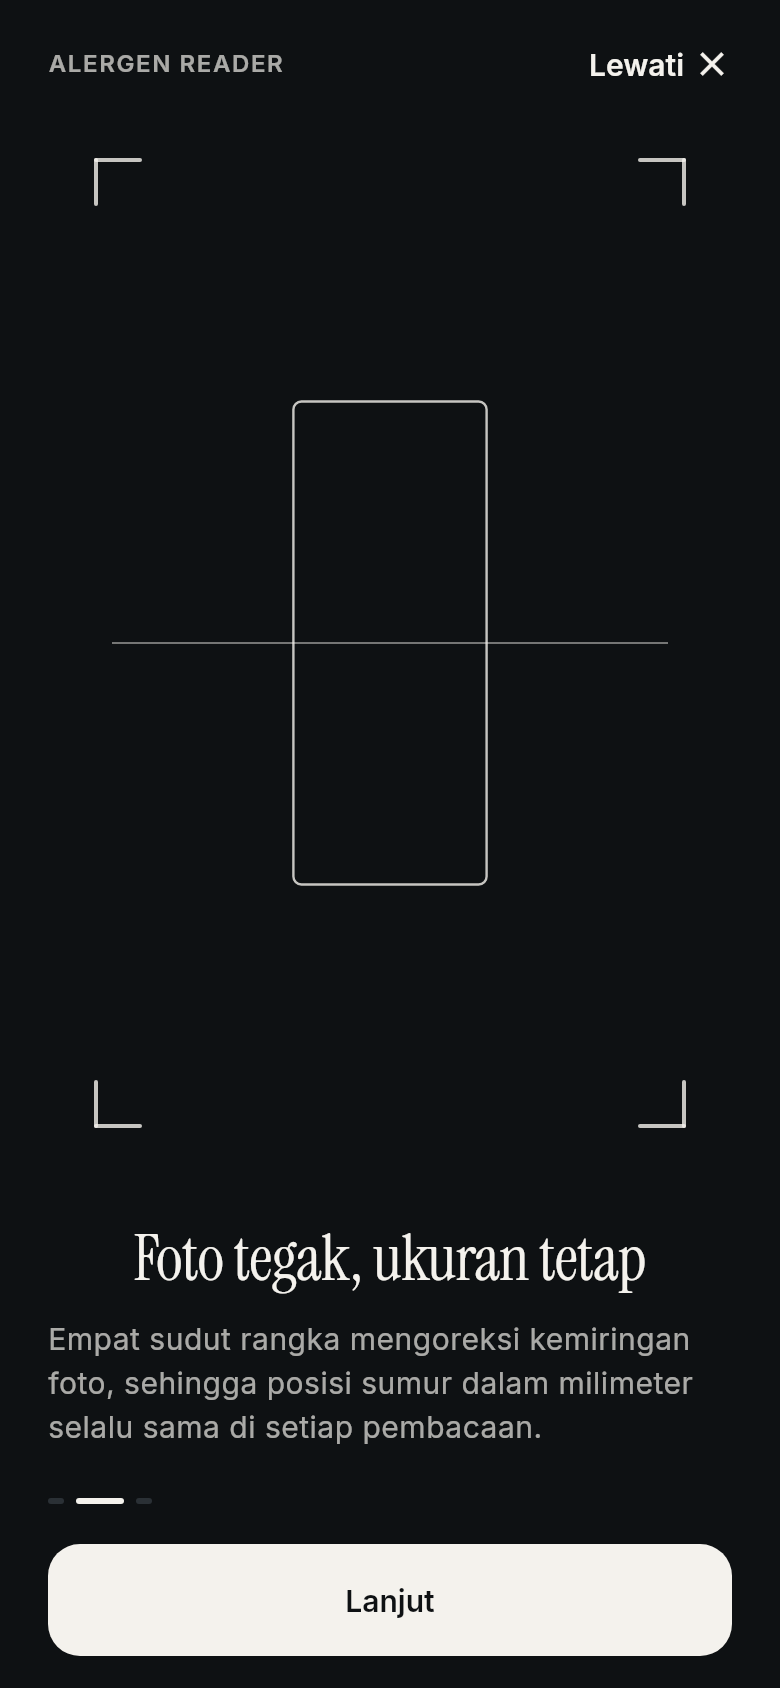
\includegraphics[width=\linewidth]{02_onboarding_2.png}
\subcaption{Halaman 2: pandangan bidik dengan empat tanda sudut dan garis horizon
mengajarkan pose kamera tegak sebelum pengguna salah mengambil foto pertama.}\label{fig:onb2}
\end{minipage}\hfill
\begin{minipage}[t]{0.30\textwidth}
\centering
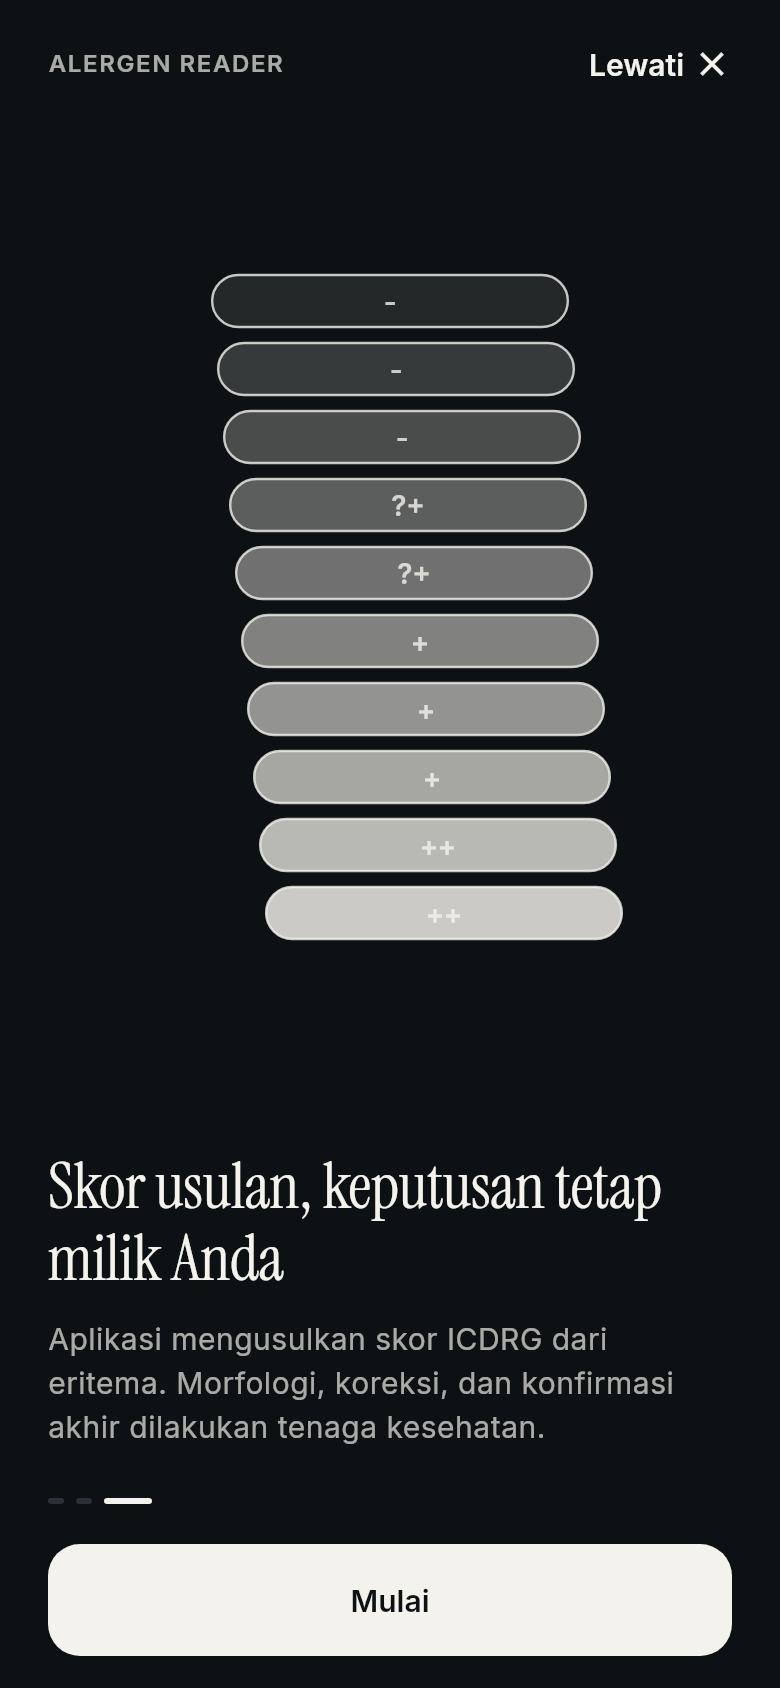
\includegraphics[width=\linewidth]{03_onboarding_3.png}
\subcaption{Halaman 3: sepuluh pil skor menaik dengan simbol ICDRG menegaskan
batas peran aplikasi: skor usulan, keputusan tetap milik tenaga kesehatan.}\label{fig:onb3}
\end{minipage}
\caption{Onboarding tiga halaman pada latar tinta. Ilustrasi garis menggantikan
foto agar pesan tentang cara kerja, bukan hasil, yang tersampaikan.}
\label{fig:onboarding}
\end{figure}

Gambar~\ref{fig:onboarding} memperlihatkan ketiga halaman. Tombol Lanjut berganti
Mulai di halaman terakhir; tautan Lewati di kanan atas selalu tersedia bagi
pengguna berulang yang membuka panduan ulang dari Pengaturan.

\subsection{Beranda}

Beranda memakai header dengan tanggal panjang Indonesia, kartu hero tinta berisi
dua angka nyata dari state (maksimum $\Delta a^*$ pembacaan terakhir dan jumlah
menunggu konfirmasi), kendali peran dua segmen, serta ringkasan tiga baris.
Ketika belum ada pembacaan, ringkasan diganti keadaan kosong dengan tiga langkah
singkat sehingga pengguna baru tahu harus mulai dari mana tanpa membaca manual.
Untuk peran pasien yang belum diizinkan melihat skor sementara, angka $\Delta a^*$
diganti jumlah pembacaan tersimpan agar kebijakan penyembunyian skor konsisten di
seluruh aplikasi.

\begin{figure}[!htbp]
\centering
\begin{minipage}[t]{0.30\textwidth}
\centering
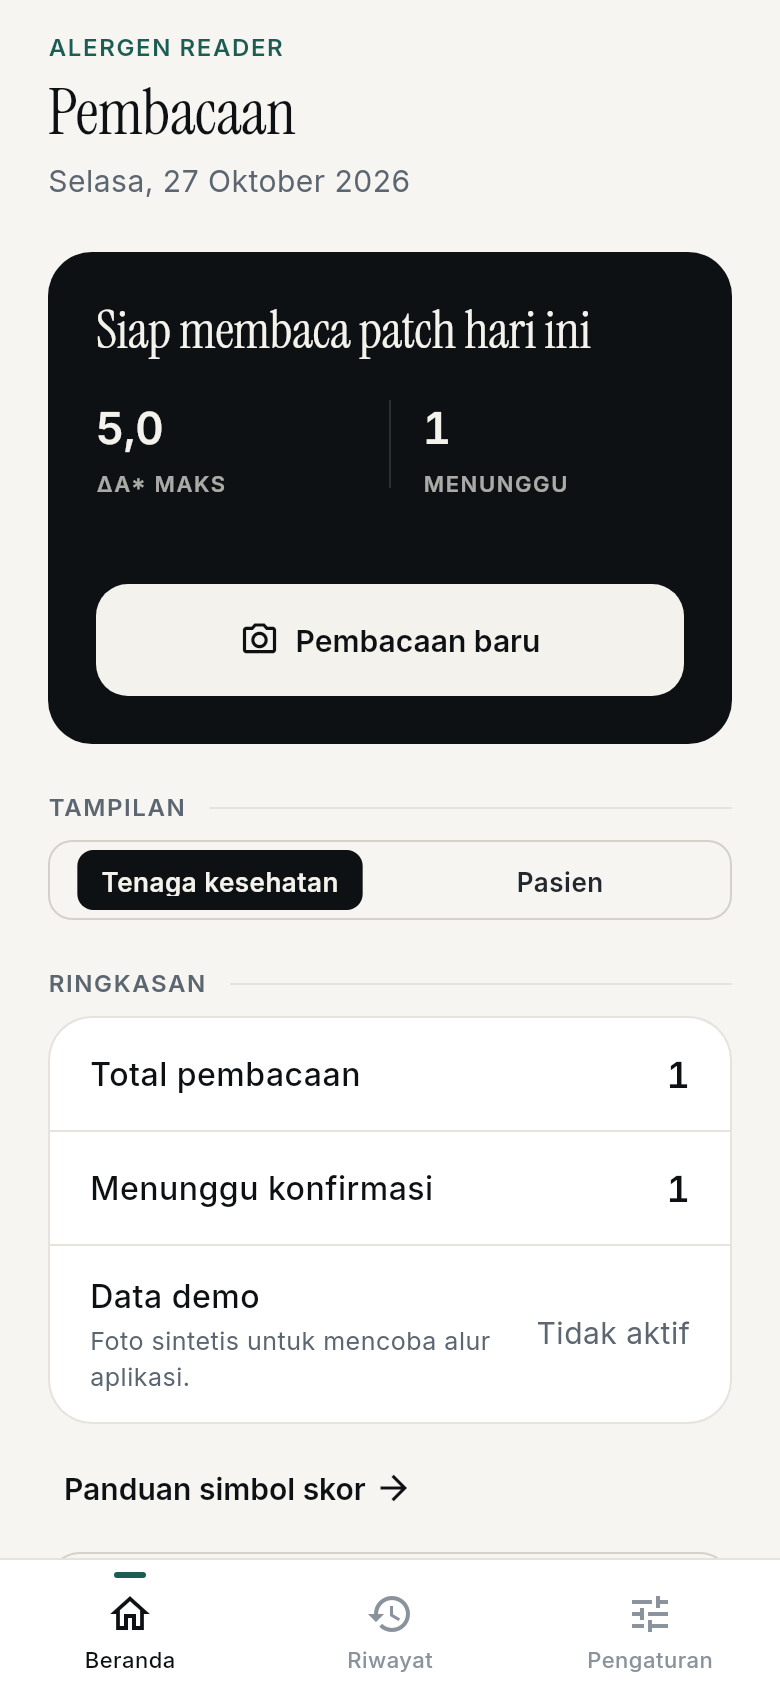
\includegraphics[width=\linewidth]{04_home.png}
\subcaption{Beranda tenaga kesehatan dengan satu pembacaan: hero tinta menampilkan
$\Delta a^*$ maksimum 5,0 dan satu pembacaan menunggu konfirmasi, diikuti kendali
peran dan ringkasan. Bilah tiga tab di bawah menandai Beranda aktif.}\label{fig:home}
\end{minipage}\hfill
\begin{minipage}[t]{0.30\textwidth}
\centering
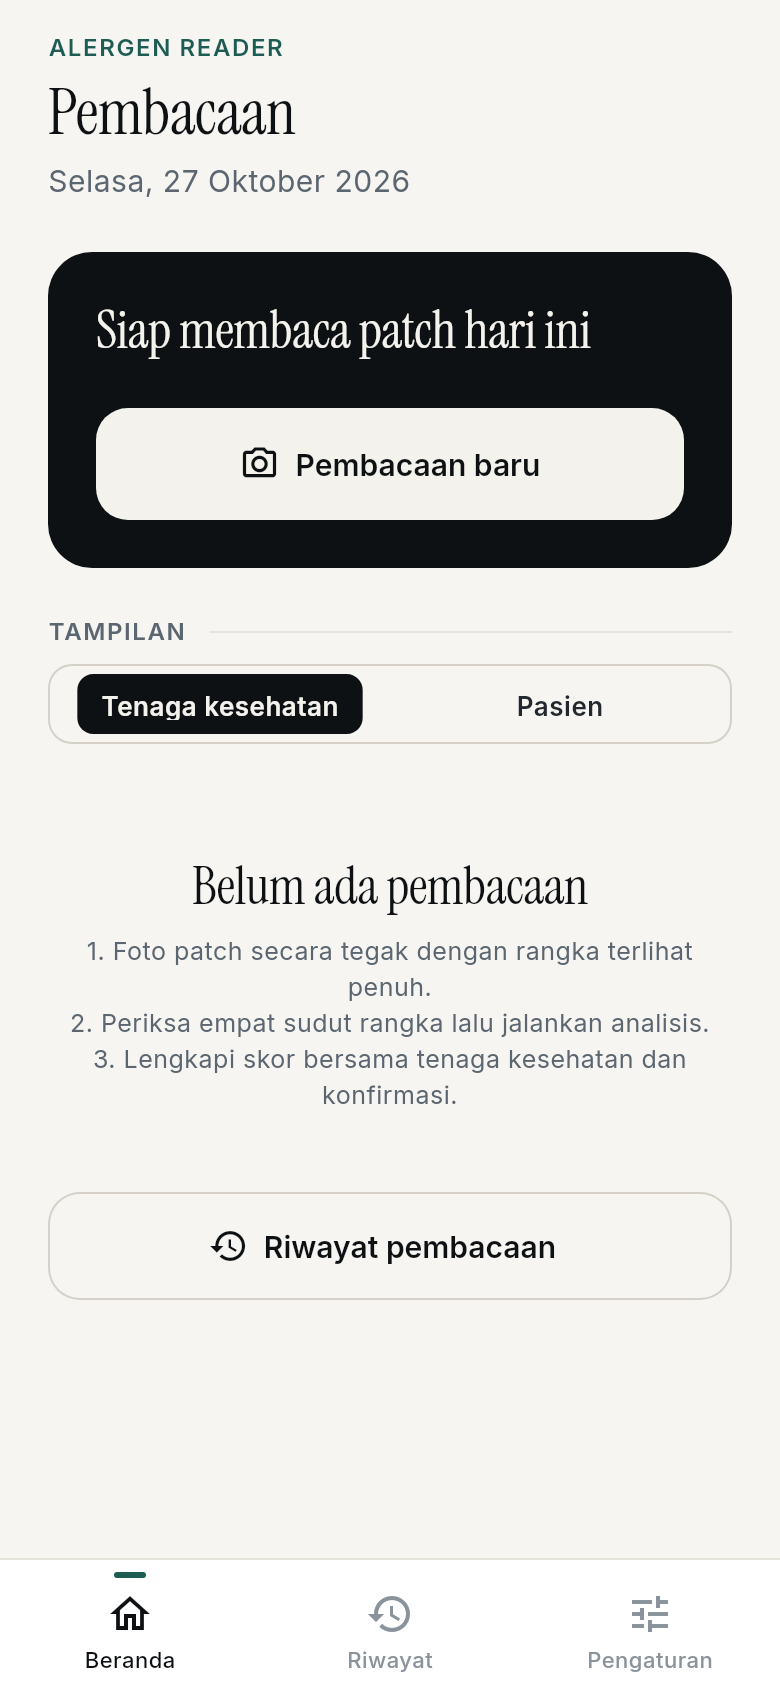
\includegraphics[width=\linewidth]{05_home_empty.png}
\subcaption{Keadaan kosong pada toko data baru: petunjuk tiga langkah (foto tegak,
periksa sudut, konfirmasi bersama tenaga kesehatan) menggantikan angka yang belum
ada.}\label{fig:homeempty}
\end{minipage}\hfill
\begin{minipage}[t]{0.30\textwidth}
\centering
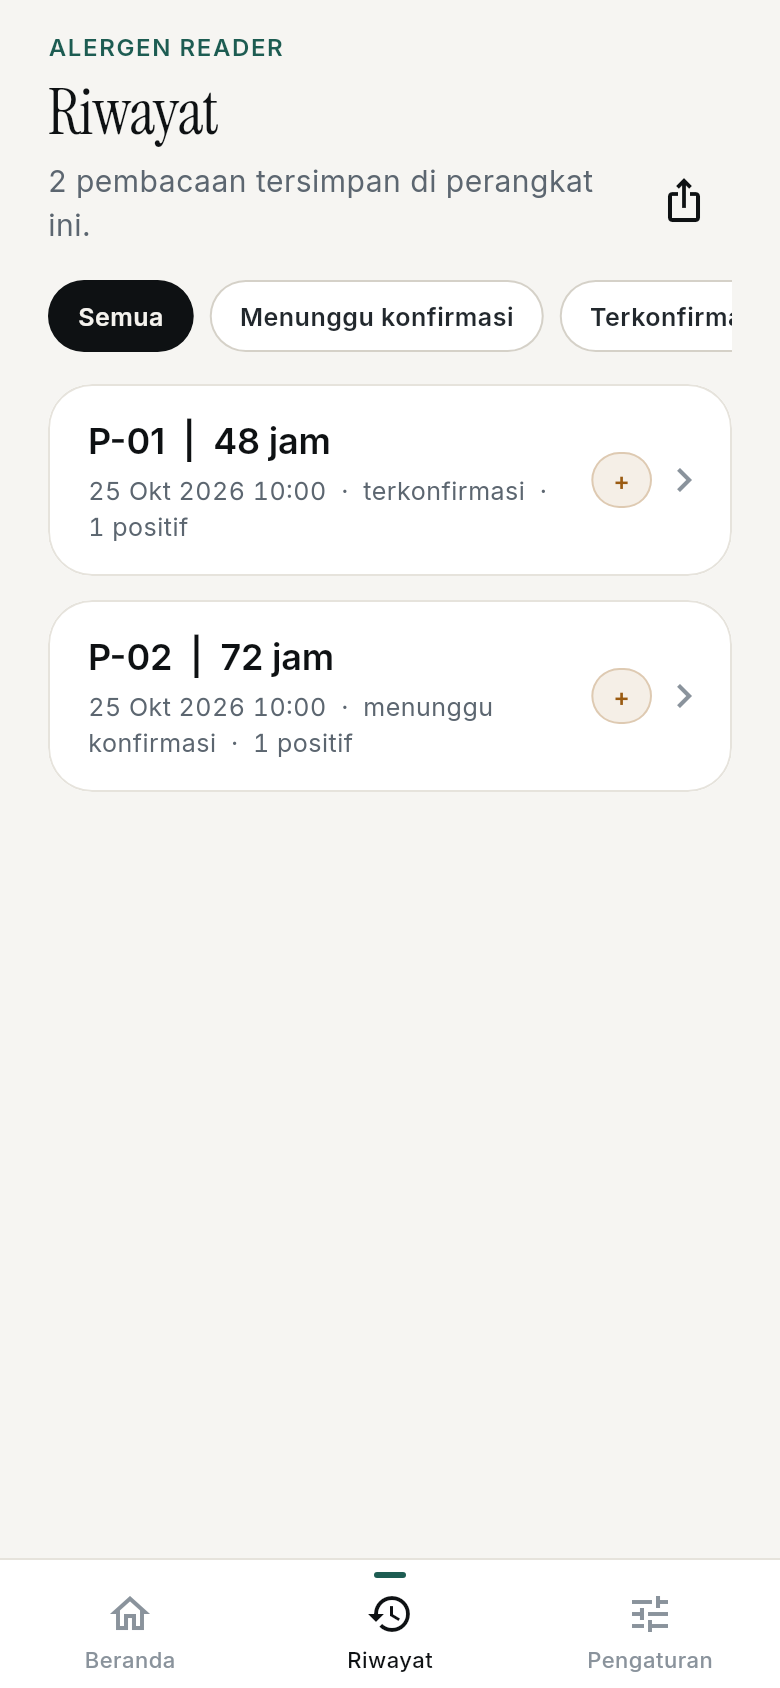
\includegraphics[width=\linewidth]{06_history.png}
\subcaption{Riwayat dalam kerangka tab kedua: chip saringan (Semua, Menunggu
konfirmasi, Terkonfirmasi, Data demo) dan kartu per pembacaan berisi kode, jam,
tanggal, status, jumlah positif, serta chip skor tertinggi.}\label{fig:history}
\end{minipage}
\caption{Tiga layar tab utama. Semua angka pada hero dan kartu berasal dari data
nyata di penyimpanan, bukan contoh tempelan, sehingga Beranda jujur tentang isi
riwayat.}
\label{fig:tiga-tab}
\end{figure}

Gambar~\ref{fig:home} sampai Gambar~\ref{fig:history} pada
Gambar~\ref{fig:tiga-tab} memperlihatkan ketiga kondisi yang paling sering
dilihat pengguna. Geser kartu riwayat ke kiri menghapus pembacaan melalui dialog
konfirmasi, perilaku yang sama dengan versi sebelum redesain dan dijaga oleh uji
widget.

\subsection{Layar hasil untuk tenaga kesehatan}

Layar hasil adalah layar terpenting aplikasi dan memakai komposisi paling padat:
banner status di atas, kartu foto terkoreksi dengan cincin warna skor dan pil
simbol tinta di atas tiap sumur, baris legenda mini tujuh simbol, MetricStrip
tiga angka ringkas, daftar sepuluh WellRow, dan bilah konfirmasi melekat di
bawah. Foto pada Gambar~\ref{fig:result} adalah foto demo nyata yang dianalisis
pipeline penuh, sehingga cincin dan pil menempel pada kulit sesungguhnya; halo
putih 5 px di bawah tiap cincin warna menjaga keterbacaan pada kulit gelap
maupun terang.

\begin{figure}[!htbp]
\centering
\begin{minipage}[t]{0.30\textwidth}
\centering
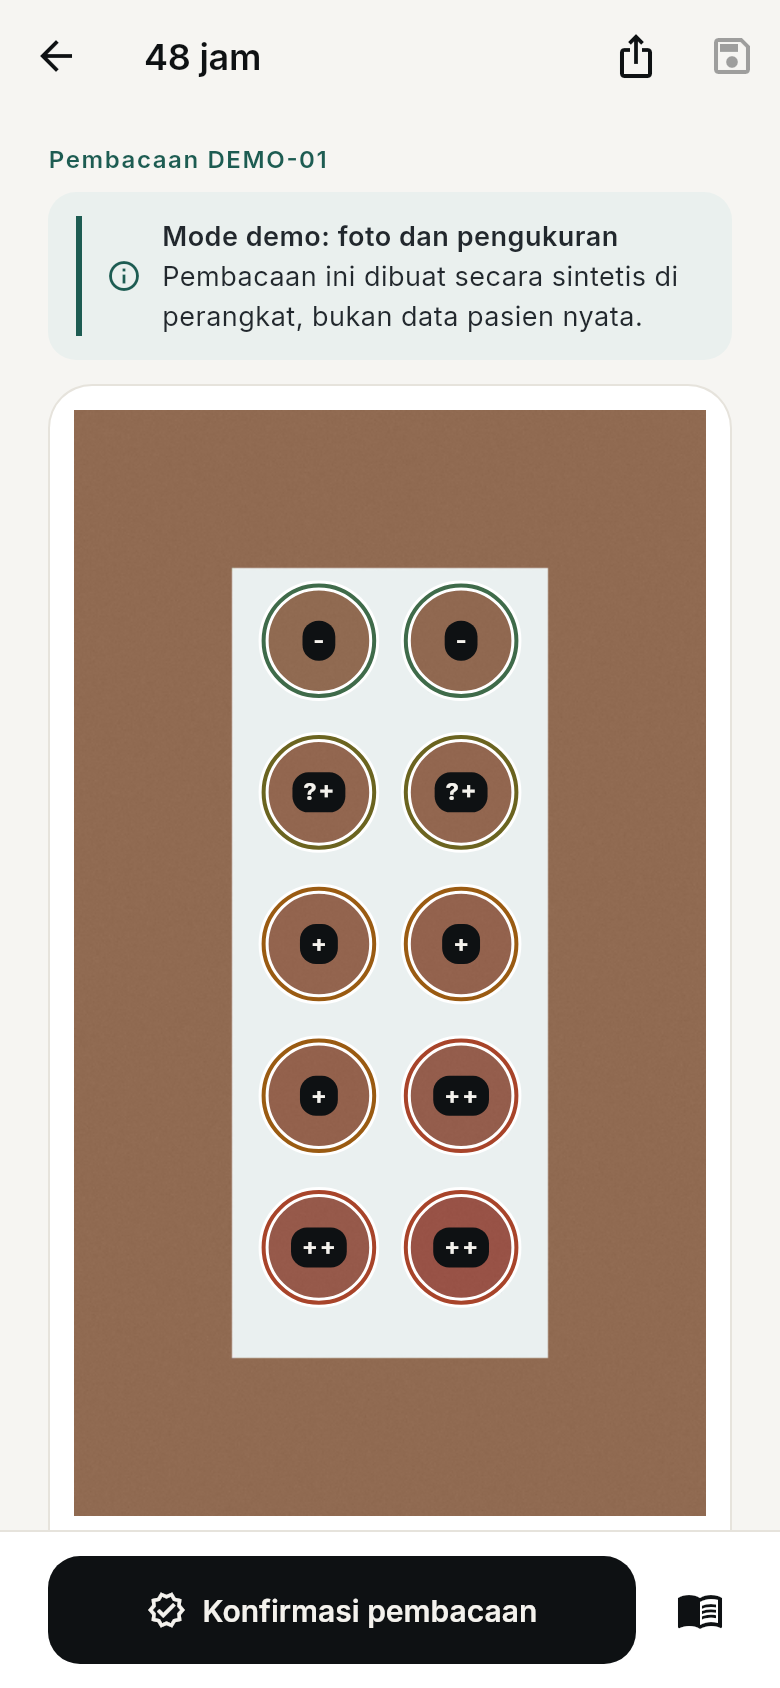
\includegraphics[width=\linewidth]{07_result.png}
\subcaption{Hasil untuk tenaga kesehatan: eyebrow kode pembacaan, banner mode
demo, foto terkoreksi dengan sepuluh pil skor tinta dan cincin warna, caption
warna kulit acuan L*a*b*, serta bilah Konfirmasi pembacaan yang melekat.}\label{fig:result}
\end{minipage}\hfill
\begin{minipage}[t]{0.30\textwidth}
\centering
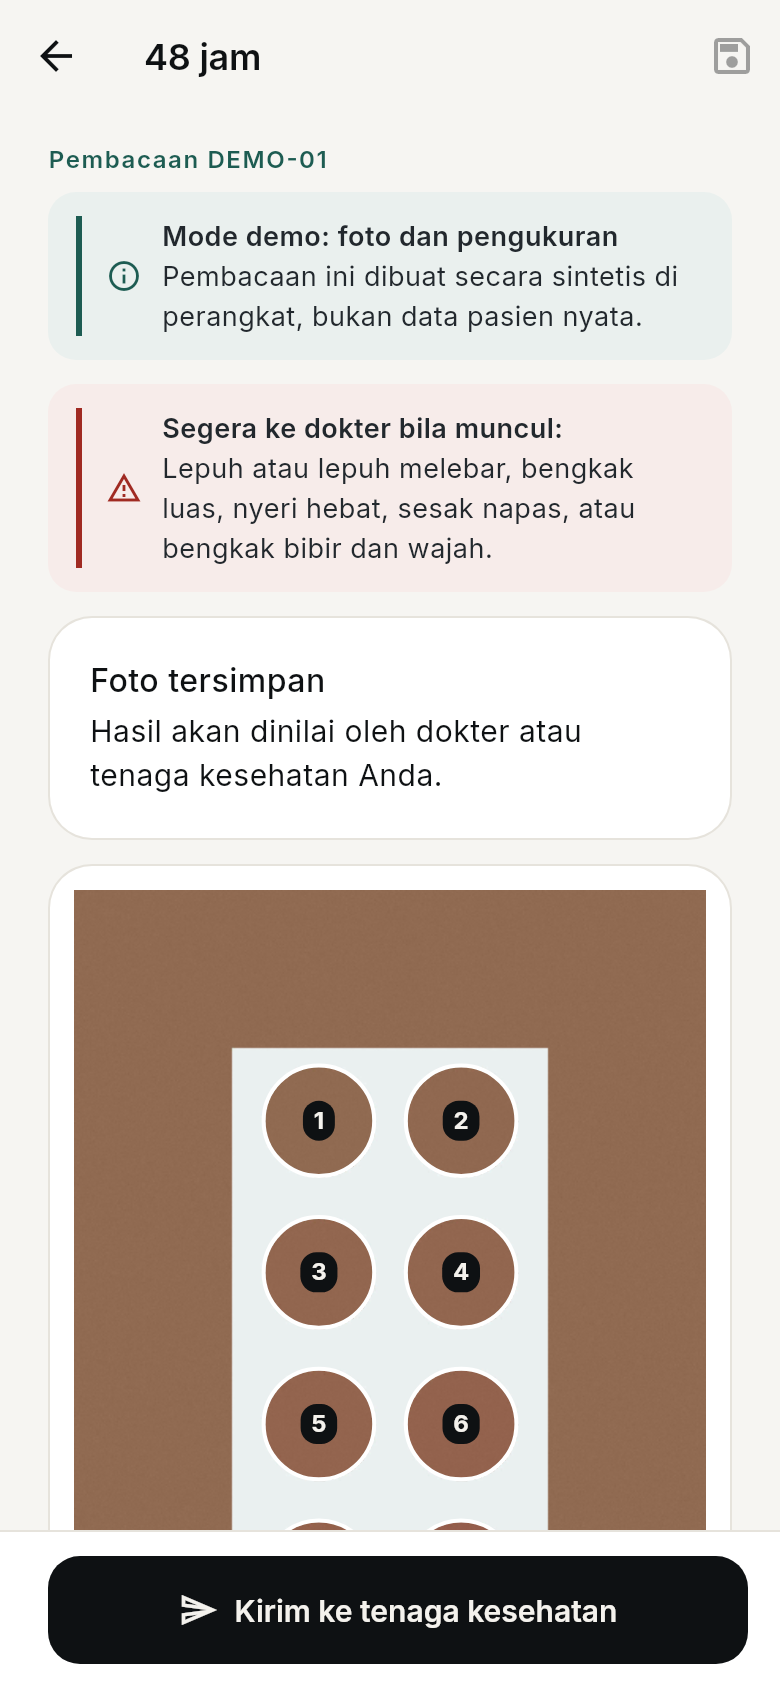
\includegraphics[width=\linewidth]{08_result_patient.png}
\subcaption{Hasil untuk pasien: tanpa skor, tanpa cincin warna, tanpa MetricStrip.
Yang tampil adalah banner tanda bahaya, kartu Foto tersimpan, foto dengan cincin
netral, dan tombol Kirim ke tenaga kesehatan.}\label{fig:patient}
\end{minipage}
\caption{Perbandingan dua peran pada pembacaan yang sama. Kebijakan penyembunyian
skor pasien diterapkan lewat struktur widget, bukan sekadar warna, sehingga uji
dapat memastikan tidak ada GradeChip maupun teks $\Delta a^*$ di pohon widget
peran pasien.}
\label{fig:hasil-dua-peran}
\end{figure}

Menggulir layar hasil menyingkap bagian yang tidak muat di layar pertama.
Gambar~\ref{fig:scroll} menampilkan MetricStrip berisi $\Delta a^*$ maksimum
6,5, dua sumur bernilai positif, dan rerata area merah 40,0\%, diikuti label
sepuluh sumur dan deretan WellRow. Setiap WellRow dapat dibuka seperti pada
Gambar~\ref{fig:expanded} untuk memperlihatkan metrik tiga kolom sumur itu,
saran otomatis, enam chip koreksi dokter, empat chip morfologi, dan aksi kembali
ke saran; ekspansi menyusun diri ke dalam pandangan lewat pengguliran otomatis
agar chip tidak pernah tertutup bilah bawah.

\begin{figure}[!htbp]
\centering
\begin{minipage}[t]{0.30\textwidth}
\centering
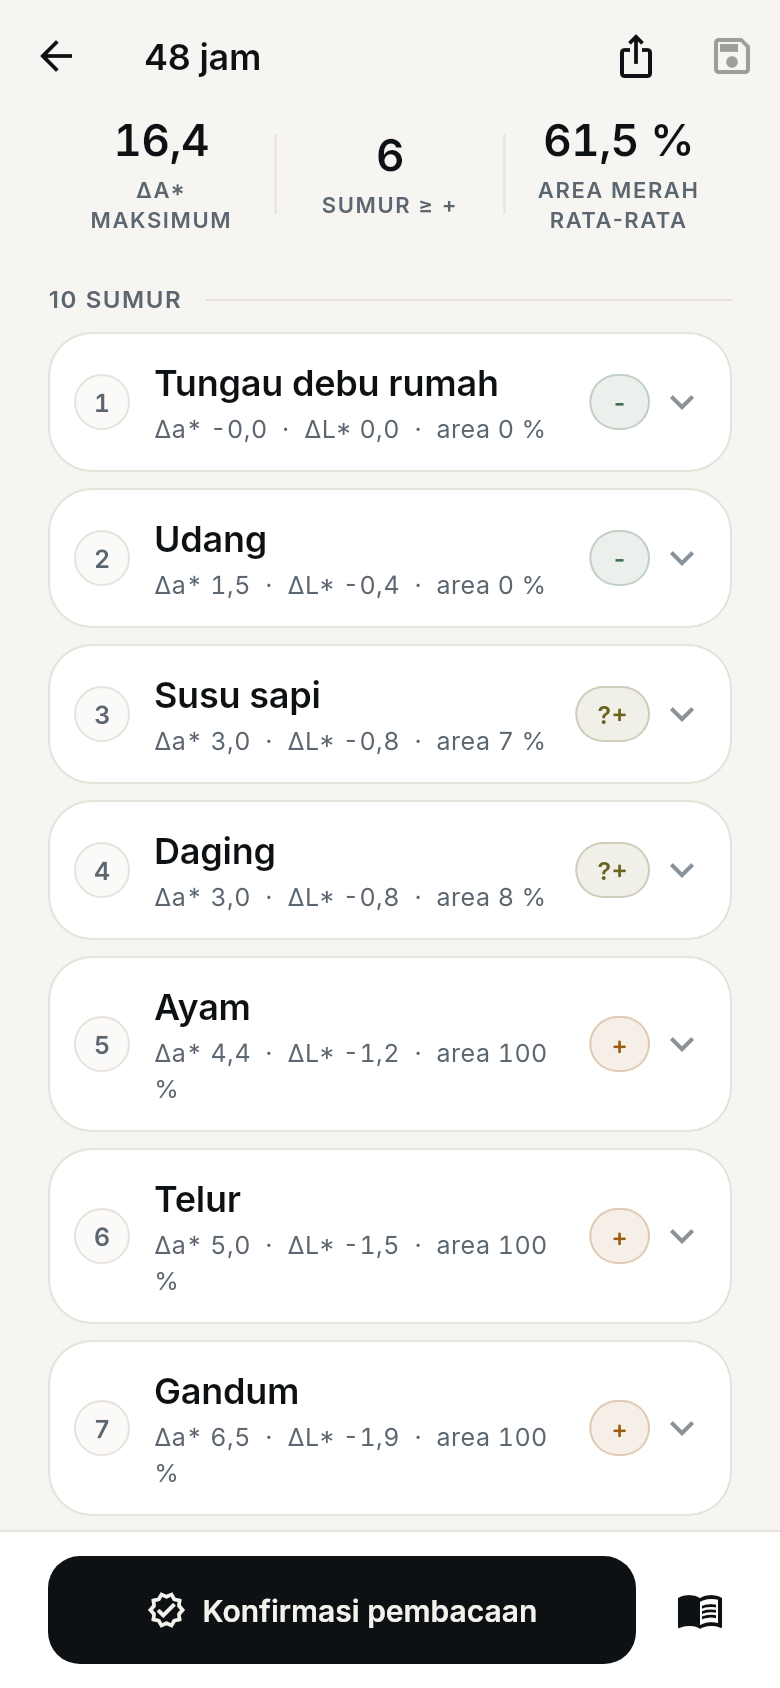
\includegraphics[width=\linewidth]{12_result_scroll.png}
\subcaption{Bagian hasil setelah digulir: MetricStrip tiga angka (maksimum
$\Delta a^*$ 6,5; dua sumur $\geq +$; rerata area merah 40,0\%), label 10 SUMUR,
dan WellRow dengan lingkar nomor, nama alergen, baris metrik, dan chip skor.}\label{fig:scroll}
\end{minipage}\hfill
\begin{minipage}[t]{0.30\textwidth}
\centering
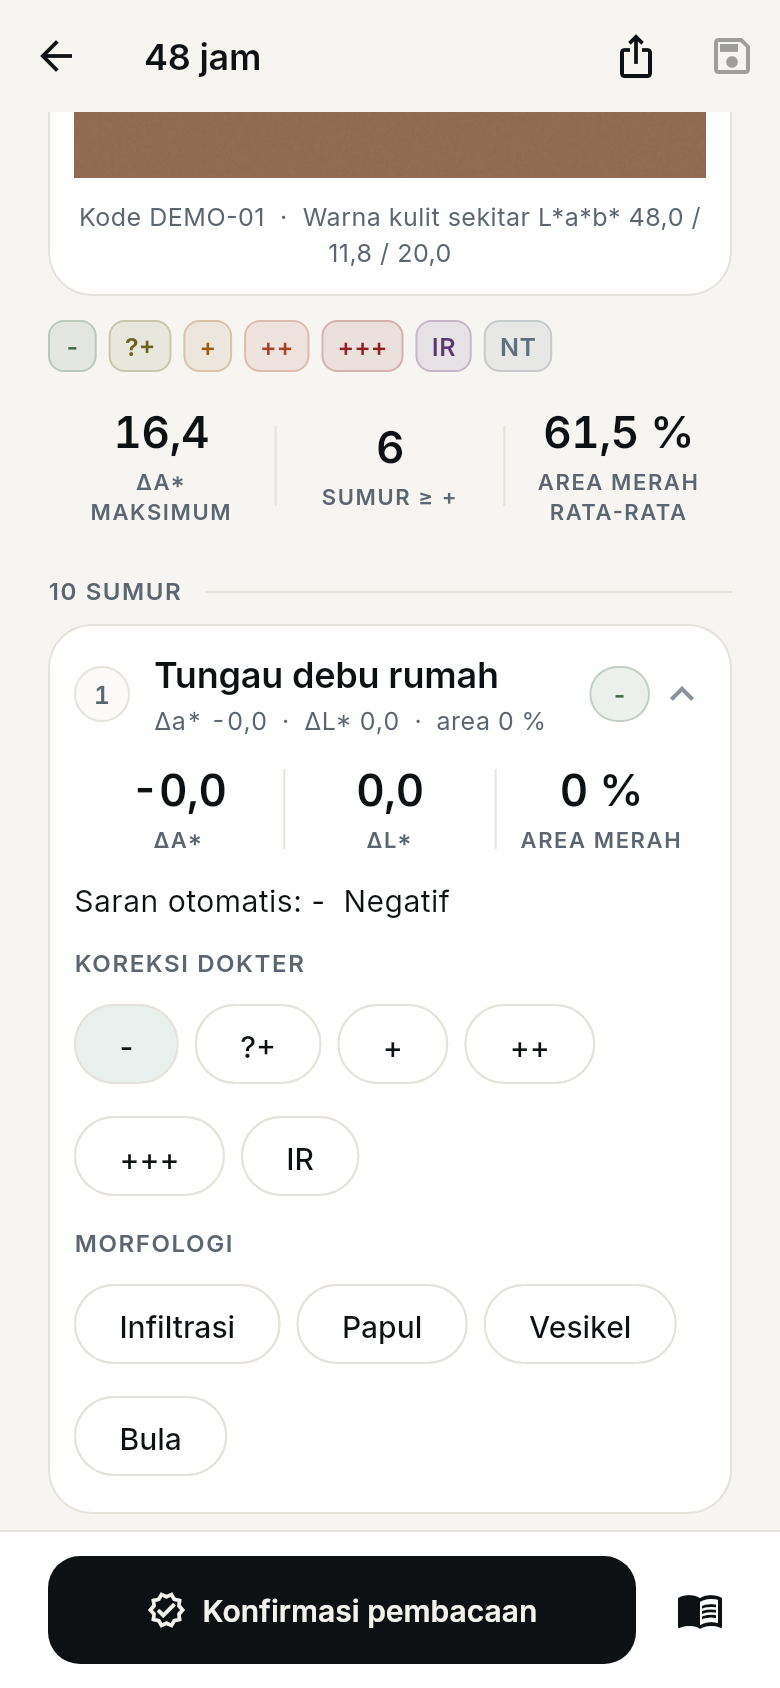
\includegraphics[width=\linewidth]{13_result_well_expanded.png}
\subcaption{Satu WellRow terbuka: metrik sumur tiga kolom, baris Saran otomatis,
chip koreksi dokter enam simbol, dan chip morfologi empat pilihan. Morfologi
hanya dapat menaikkan saran; kembali ke saran membatalkan timpaan.}\label{fig:expanded}
\end{minipage}
\caption{Detail layar hasil. Chip memakai komponen Material asli dengan gaya
tema sehingga perilaku sentuh, fokus, dan aksesibilitasnya standar.}
\label{fig:hasil-detail}
\end{figure}

\subsection{Pengaturan dan legenda skor}

Pengaturan dikelompokkan dalam seksi berlabel: konfigurasi aktif (rangka,
diameter sumur, resolusi analisis, jam pembacaan, daftar sepuluh sumur dua kolom,
indikator bila memakai nilai bawaan), tampilan pasien, ekspor data, data demo,
panduan, dan tentang. Konfigurasi sengaja hanya ditampilkan, tidak diedit, karena
berkasnya dikelola klinik di luar aplikasi. Sheet legenda skor menjelaskan makna
ketujuh simbol beserta rentang $\Delta a^*$ pada Fitzpatrick IV dan catatan bahwa
ambang belum tervalidasi klinis; sheet ini dapat dibuka dari Beranda maupun bilah
bawah layar hasil.

\begin{figure}[!htbp]
\centering
\begin{minipage}[t]{0.30\textwidth}
\centering
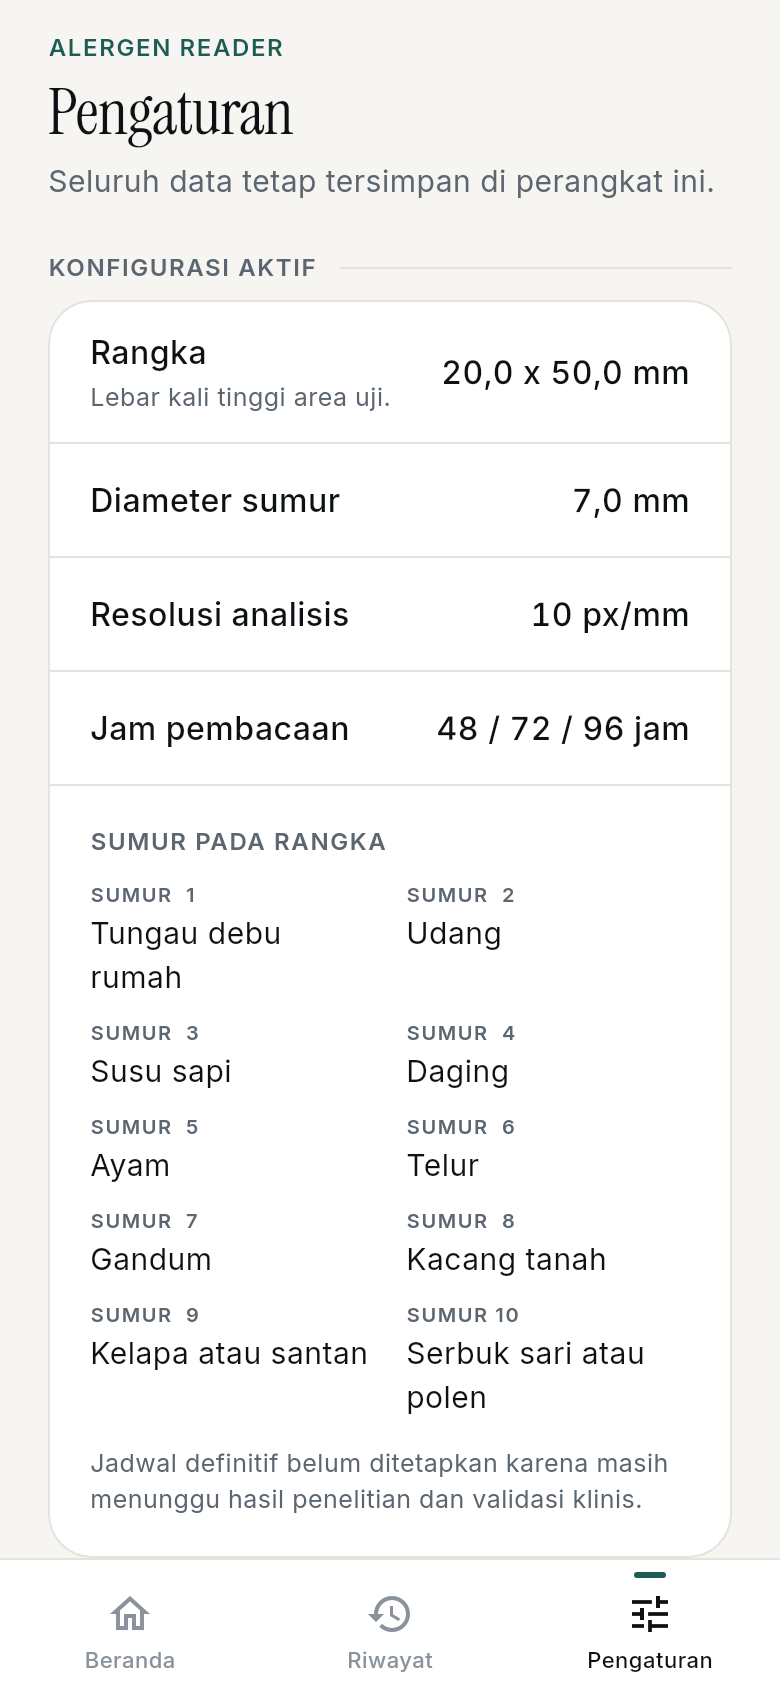
\includegraphics[width=\linewidth]{09_settings.png}
\subcaption{Pengaturan pada tab ketiga: konfigurasi aktif dengan baris kunci
nilai dan daftar sumur dua kolom, sakelar tampilan pasien, ekspor CSV, aksi data
demo, panduan, dan versi aplikasi.}\label{fig:settings}
\end{minipage}\hfill
\begin{minipage}[t]{0.30\textwidth}
\centering
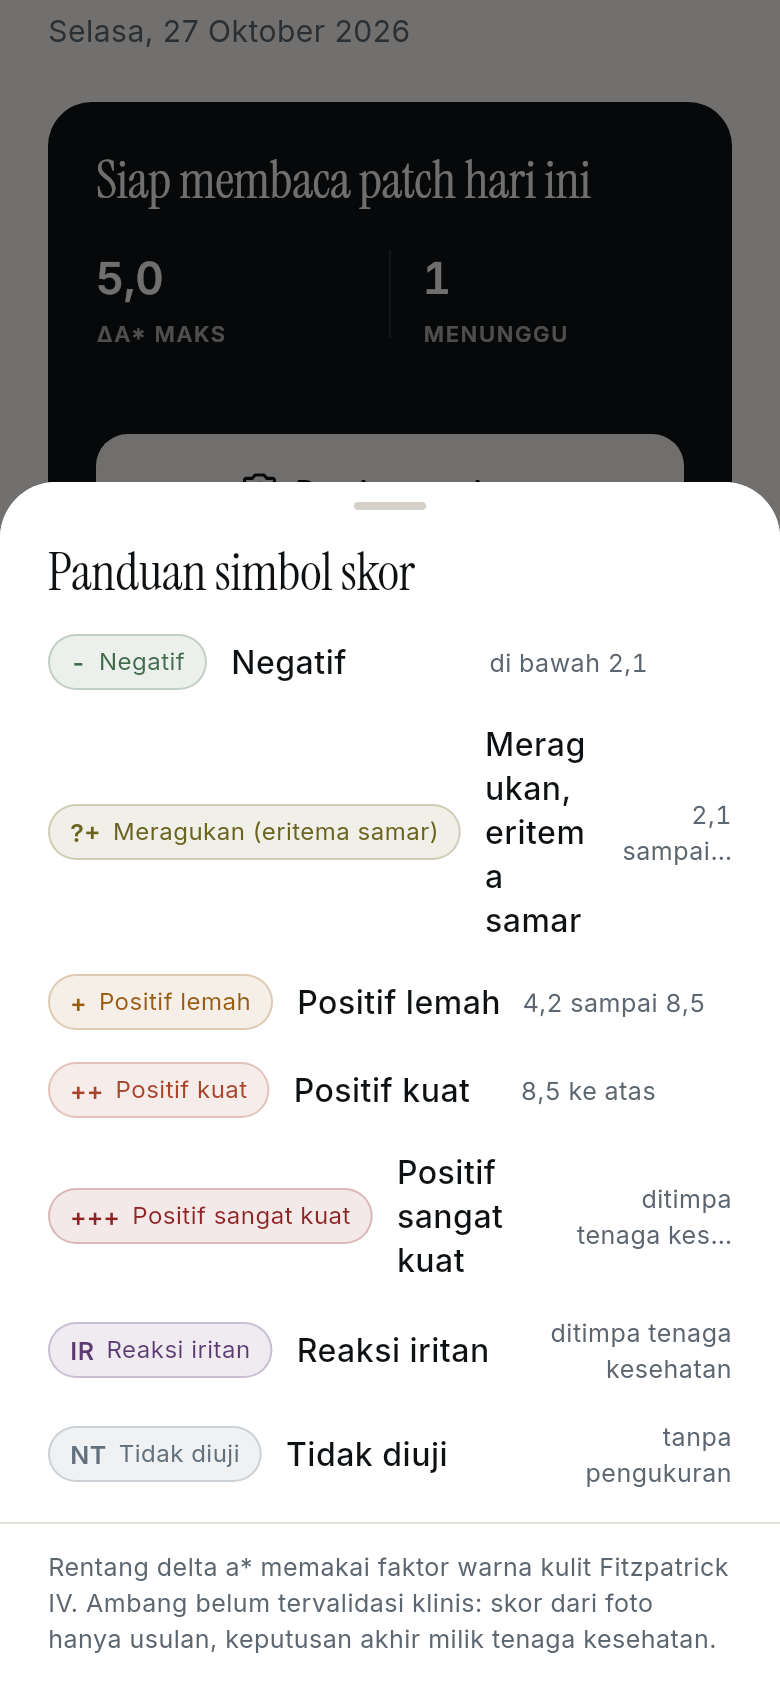
\includegraphics[width=\linewidth]{10_legend.png}
\subcaption{Sheet Panduan simbol skor di atas Beranda: tujuh baris simbol dengan
makna dan rentang $\Delta a^*$ Fitzpatrick IV, ditutup catatan bahwa skor foto
hanyalah usulan.}\label{fig:legend}
\end{minipage}
\caption{Pengaturan dan legenda. Legenda sengaja berupa sheet, bukan halaman,
agar dapat dikonsultasikan cepat sambil melihat layar hasil.}
\label{fig:settings-legend}
\end{figure}

\subsection{Skala teks besar}

Seluruh layar dirancang untuk tetap utuh ketika pengguna memperbesar teks 1,3
kali. Gambar~\ref{fig:textscaler} membandingkan Beranda pada skala normal dan
skala 1,3: hero, kendali peran, dan ringkasan melipat ke bawah tanpa teks
terpotong. Angka dan tanggal memakai angka tabular sehingga kolom tetap sejajar
pada ukuran apa pun.

\begin{figure}[!htbp]
\centering
\begin{minipage}[t]{0.30\textwidth}
\centering
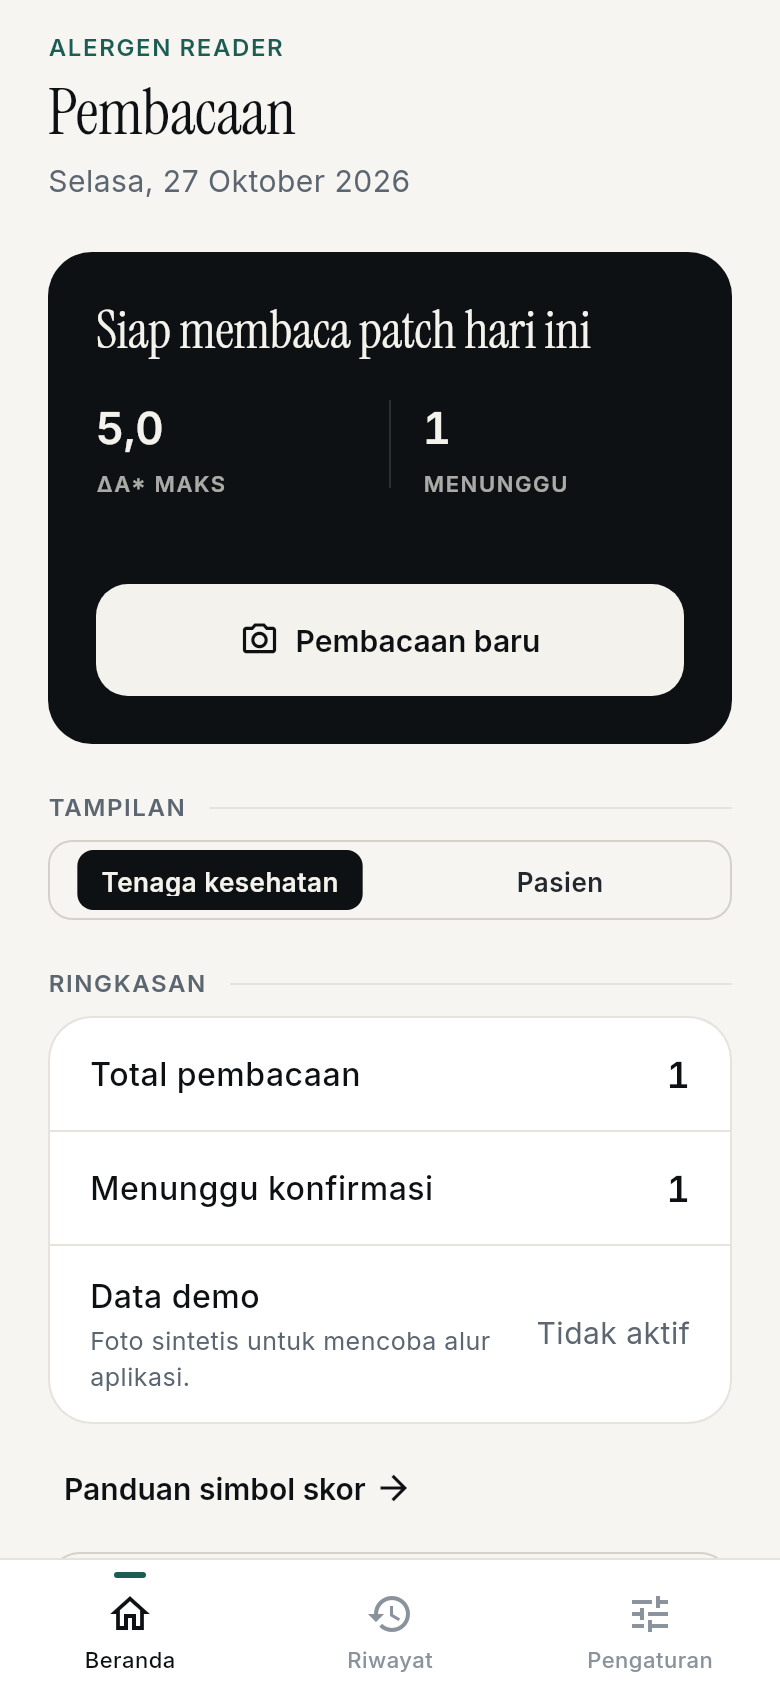
\includegraphics[width=\linewidth]{04_home.png}
\subcaption{Beranda pada skala teks normal: acuan pembanding dengan hero, kendali
peran, dan ringkasan yang sama.}\label{fig:textscaler-normal}
\end{minipage}\hfill
\begin{minipage}[t]{0.30\textwidth}
\centering
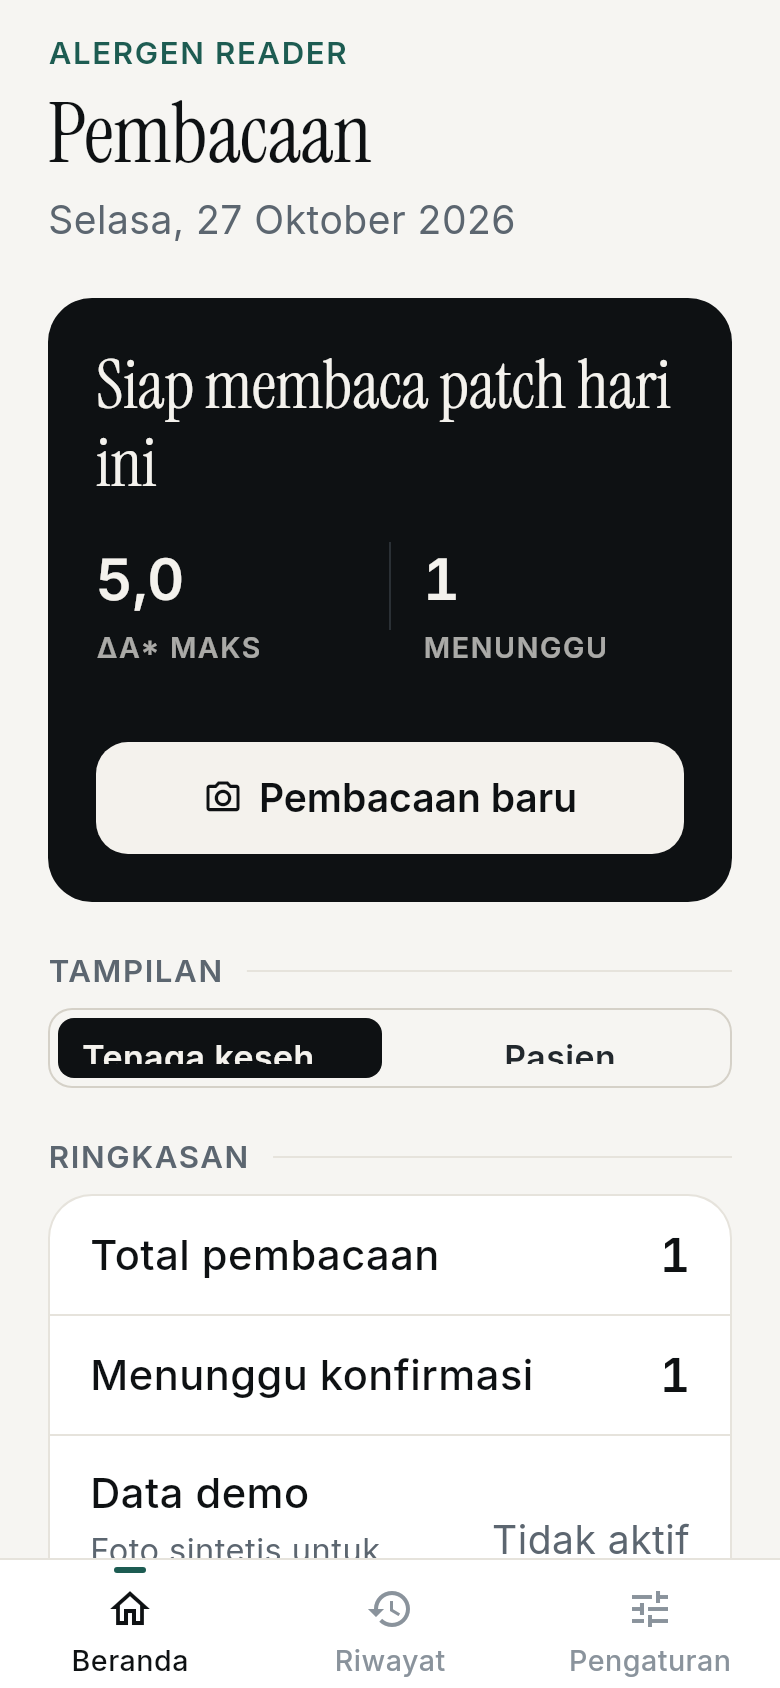
\includegraphics[width=\linewidth]{11_home_textscaler13.png}
\subcaption{Beranda pada \textit{textScaler} 1,3: seluruh baris melipat ke bawah,
tanpa teks terpotong; verifikasi otomatis 360\,x\,640 memastikan keenam layar
utama bebas \textit{overflow} pada skala ini.}\label{fig:textscaler-big}
\end{minipage}
\caption{Perbandingan Beranda pada skala teks normal dan 1,3 pada 390\,x\,844.
Perbesaran teks menggeser tinggi baris, bukan memotongnya, karena seluruh
kontainer melipat mengikuti ukuran fon.}
\label{fig:textscaler}
\end{figure}

% ============================ BAB 5 ============================
\section{Aksesibilitas}

\subsection{Prinsip yang dijalankan}

Empat prinsip dijalankan sekaligus di kode dan diuji otomatis. Pertama, skala
teks: keenam layar utama dirender pada 360\,x\,640 piksel dengan skala teks 1,3
oleh \texttt{a11y\_test.dart}, dan setiap \textit{exception} layout akan
menggagalkan uji. Kedua, kejelasan huruf: Inter dan Instrument Serif dibundel di
\texttt{assets/fonts} sehingga tidak ada kotak pengganti (\textit{tofu}) pada
perangkat tanpa fon sistem; uji khusus membaca fon terpakai dari paragraf yang
dirender dan memastikan keluarganya Inter. Ketiga, kontras: pasangan teks dan
latar pada palet Clinical Ink memenuhi rasio 4,5:1 untuk teks ukuran baca, dan
warna tidak pernah menjadi satu-satunya pembawa makna skor karena selalu disertai
simbol dan label. Keempat, semantik: ikon aksi memiliki label Indonesia, pil skor
di foto diberi label semantik per sumur, dan label skor tidak pernah bocor ke
pohon semantik peran pasien.

\subsection{Ringkasan uji dan hasilnya}

\begin{table}[H]
\centering
\caption{Uji aksesibilitas pada test/a11y\_test.dart dan hasilnya.}
\label{tab:a11y}
\tabstart
\begin{tabular}{@{}L{7.2cm}L{7.0cm}@{}}
\toprule
\hdrrow\tH{Uji} & \tH{Hasil} \\
\midrule
\tcell{Onboarding pada 360\,x\,640, skala 1,3} & \tcell{Lulus tanpa \textit{overflow}.} \\
\tcell{Beranda kedua peran, skala 1,3} & \tcell{Lulus untuk tenaga kesehatan dan pasien.} \\
\tcell{Riwayat dua pembacaan, skala 1,3} & \tcell{Lulus; kartu dan chip saringan utuh.} \\
\tcell{Hasil tenaga kesehatan, skala 1,3} & \tcell{Lulus; ekspansi WellRow menyusun diri ke pandangan.} \\
\tcell{Hasil pasien, skala 1,3} & \tcell{Lulus; tanpa elemen skor di pohon widget.} \\
\tcell{Pengaturan, skala 1,3} & \tcell{Lulus; daftar sumur dua kolom utuh.} \\
\tcell{Label tombol pasien utuh pada 360 px} & \tcell{Lulus; tepi kanan label terukur dalam layar.} \\
\bottomrule
\end{tabular}
\end{table}

Seluruh baris pada Tabel~\ref{tab:a11y} berstatus lulus pada build 0.2.0.
Pemeriksaan label tombol pasien ditambahkan setelah tinjauan tangkapan layar
menemukan teks terpotong; label kini diperpendek dan uji memastikan batas kanan
teks tetap di dalam layar.

% ============================ BAB 6 ============================
\section{Pengujian dan Verifikasi}

\subsection{Susunan uji}

\begin{table}[H]
\centering
\caption{Berkas uji dan yang dikunci.}
\label{tab:uji}
\tabstart
\begin{tabular}{@{}L{4.4cm}L{9.8cm}@{}}
\toprule
\hdrrow\tH{Berkas} & \tH{Yang diverifikasi} \\
\midrule
\tcell{analyzer\_test.dart} & \tcell{Pipeline citra pada kanvas sintetis:
geometri, metrik $\Delta a^*/\Delta L^*$, kualitas.} \\
\tcell{grading\_test.dart} & \tcell{Pemetaan skor, lantai morfologi, faktor
Fitzpatrick, gabungan timpaan.} \\
\tcell{csv\_export\_test.dart} & \tcell{Format CSV 31 baris untuk 3 sesi dan
penguraian ulang.} \\
\tcell{config\_test.dart} & \tcell{Konfigurasi rusak jatuh ke nilai bawaan tanpa
crash.} \\
\tcell{demo\_seed\_test.dart} & \tcell{Tiga sesi demo melalui pipeline nyata,
CSV 41 baris bercampur data nyata, hapus demo tak menyentuh data nyata.} \\
\tcell{onboarding\_test.dart} & \tcell{Tiga halaman, tombol Lanjut/Mulai/Lewati,
sheet legenda tujuh simbol dengan metrik fon nyata.} \\
\tcell{widgets\_test.dart} & \tcell{Timpaan dokter, morfologi hanya menaikkan,
peran pasien, konfirmasi, banner kualitas, fon anti-tofu, riwayat dan hapus.} \\
\tcell{a11y\_test.dart} & \tcell{Enam layar pada 360\,x\,640 skala 1,3 dan label
tombol pasien.} \\
\tcell{tool/screenshots\_test.dart} & \tcell{Tiga belas tangkapan layar 390\,x\,844
DPR 2 dengan fon asli; bukti visual dokumen ini.} \\
\bottomrule
\end{tabular}
\end{table}

Perintah \texttt{flutter test} menjalankan 45 uji pada delapan berkas di folder
\texttt{test}; harness screenshot berjalan terpisah dengan
\texttt{flutter test tool/screenshots\_test.dart}. Semuanya lulus pada build
yang didokumentasikan, dan analisis statis \texttt{flutter analyze} bersih tanpa
keluhan.

\subsection{Harness tangkapan layar}

Harness merender tiap layar pada 390\,x\,844 piksel logis dengan rasio piksel
perangkat 2, memuat fon Inter dan Instrument Serif asli lewat FontLoader, serta
fon ikon Material dari pohon SDK karena keduanya bukan aset aplikasi. Layar hasil
memakai foto demo yang dibangkitkan lalu dianalisis pipeline sungguhan pada saat
uji berjalan; harness menunggu kanvas foto selesai didekode sebelum menangkap.
Antar tangkapan, pohon widget dibongkar dahulu supaya keadaan berstatus (tab
aktif, rute yang terdorong) tidak bocor ke gambar berikutnya. Banner debug
dimatikan sehingga bukti visual bersih tanpa retusan.

\subsection{Gerbang kualitas dan reproduksi}

\begin{table}[H]
\centering
\caption{Gerbang kualitas dan cara mereproduksinya.}
\label{tab:gate}
\tabstart
\begin{tabular}{@{}L{5.6cm}L{8.6cm}@{}}
\toprule
\hdrrow\tH{Gerbang} & \tH{Perintah dan hasil} \\
\midrule
\tcell{Analisis statis} & \tcell{\texttt{flutter analyze}: No issues found.} \\
\tcell{Uji unit dan widget} & \tcell{\texttt{flutter test}: 45/45 lulus.} \\
\tcell{Bukti visual} & \tcell{\texttt{flutter test tool/screenshots\_test.dart}:
13 PNG di \texttt{shots/}.} \\
\tcell{Build rilis} & \tcell{\texttt{flutter build apk --release -{}-split-per-abi}:
sukses, ukuran pada Tabel~\ref{tab:apk}.} \\
\tcell{Uji silang Python} & \tcell{\texttt{python3 tools/synthetic\_test.py}:
galat maksimum $\Delta a^*$ 0,19 pada uji sintetis.} \\
\bottomrule
\end{tabular}
\end{table}

Seluruh gerbang dijalankan ulang setiap kali perubahan antarmuka di-commit; pada
0.2.0 keenam gerbang hijau sebagaimana dicatat pada laporan redesain di
\texttt{docs/REDESIGN-REPORT.md}.

% ============================ BAB 7 ============================
\section{Build dan Rilis}

\subsection{Perintah build}

Build rilis Android dipisah per ABI agar ukuran unduhan minimal:
\begin{quote}
\small\texttt{export JAVA\_HOME=/usr/lib/jvm/java-21-openjdk-amd64}\\
\small\texttt{export ANDROID\_HOME=\$HOME/Android}\\
\small\texttt{flutter build apk --release --split-per-abi}
\end{quote}
Keluaran berada di \texttt{build/app/outputs/flutter-apk/}. Lingkungan yang
dipakai adalah Flutter 3.44.8 dengan Dart 3.12.2, Gradle 8.4, AGP 8.2.2, dan
Kotlin 1.9.22; peningkatan versi build tidak dilakukan selama siklus 0.2.0 demi
stabilitas reproduksi.

\begin{table}[H]
\centering
\caption{Keluaran build rilis 0.2.0 per ABI.}
\label{tab:apk}
\tabstart
\begin{tabular}{@{}L{7.0cm}L{3.2cm}L{4.0cm}@{}}
\toprule
\hdrrow\tH{Berkas APK} & \tH{Ukuran} & \tH{Catatan} \\
\midrule
\tcell{app-armeabi-v7a-release.apk} & \tcell{18,9 MB} & \tcell{Perangkat 32 bit ARM.} \\
\tcell{app-arm64-v8a-release.apk} & \tcell{21,0 MB} & \tcell{Perangkat 64 bit umum; melebihi ambang 15 MB.} \\
\tcell{app-x86\_64-release.apk} & \tcell{22,5 MB} & \tcell{Emulator dan perangkat x86.} \\
\bottomrule
\end{tabular}
\end{table}

Fon Inter dan Instrument Serif terbundel penuh di dalam APK, sementara fon ikon
Material di-\textit{tree-shake} dari 1,6 MB menjadi sekitar 4 KB karena hanya
ikon yang dipakai yang disertakan.

\subsection{Verifikasi setelah build}

Setelah build, verifikasi minimum yang dijalankan: ketiga berkas APK ada dan
ukurannya masuk akal; \texttt{flutter analyze} tetap bersih; seluruh uji tetap
lulus; dan harness screenshot masih menghasilkan 13 berkas yang sama sehingga
perilaku visual tidak berubah oleh proses build. Untuk perangkat iOS, dua izin
kamera perlu ditambahkan pada Info.plist sebelum build perangkat, yaitu
\texttt{NSCameraUsageDescription} dan \texttt{NSPhotoLibraryUsageDescription};
izin kamera Android sudah dideklarasikan di manifes.

% ============================ BAB 8 ============================
\section{Batasan dan Pekerjaan Lanjutan}

\subsection{Yang belum ada}

\begin{itemize}
\item \textbf{Validasi klinis.} Ambang $\Delta a^*$ 2,5 / 5 / 10, faktor
Fitzpatrick, dan ambang ketajaman belum diuji terhadap penilaian dokter;
jadwal pembacaan definitif menunggu hasil penelitian.
\item \textbf{Uji perangkat nyata.} Kamera, izin, dan alur di ponsel fisik belum
dijalankan; verifikasi sejauh ini lewat analisis statis, uji widget, dan build.
\item \textbf{Privasi lanjutan.} Enkripsi penyimpanan, kunci perangkat,
persetujuan tertulis, dan kebijakan retensi sesuai UU PDP belum ada; versi ini
sepenuhnya lokal di perangkat.
\item \textbf{Keterbatasan pada kulit gelap.} Eritema kurang terbaca lewat
kanal a*; metrik tambahan seperti indeks eritema dari saluran hijau menjadi
kandidat penelitian.
\item \textbf{Rangka fisik.} Rangka cetak 3D yang ada menutup sumur dengan
plastik; pembacaan memerlukan rangka berjendela terbuka, dan koordinat sumur
masih hasil pengukuran foto, belum dari berkas CAD.
\end{itemize}

\subsection{Rencana kerja berikutnya}

Validasi klinis mengikuti rencana pada spesifikasi: kumpulkan sedikitnya 200
sumur berlabel dari dua dokter kulit independen dengan sebaran Fitzpatrick III
sampai V, kalibrasi ambang lewat kurva ROC per kelompok warna kulit, uji cahaya
dan antarperangkat 3 sampai 5 ponsel, lalu konsultasi status regulasi karena
perangkat lunak yang memengaruhi keputusan klinis berpotensi tergolong alat
kesehatan. Pada jalur produk, tahap berikutnya adalah laporan PDF per pasien,
perbandingan 48 dan 72 jam berdampingan, kaca pembesar pada pemilih sudut,
kemudian sinkronisasi server dan model terlatih setelah data berlabel cukup.

% ============================ LAMPIRAN A ============================
\appendix
\section{Daftar Berkas Penting}

{\tabstart
\begin{longtable}{@{}L{6.3cm}L{7.9cm}@{}}
\caption{Berkas penting beserta perannya.}
\label{tab:berkas}\\
\toprule
\hdrrow\tH{Berkas} & \tH{Peran} \\
\midrule
\endfirsthead
\toprule
\hdrrow\tH{Berkas} & \tH{Peran} \\
\midrule
\endhead
\bottomrule
\endlastfoot
\tcell{lib/core/photo\_prep.dart} & \tcell{Praproses foto dan deteksi sudut rangka.} \\
\tcell{lib/core/homography.dart} & \tcell{Rektifikasi empat titik ke kanvas mm.} \\
\tcell{lib/core/skin\_analyzer.dart} & \tcell{Analisis per sumur dan cek kualitas.} \\
\tcell{lib/core/grading.dart} & \tcell{Ambang skor, morfologi, Fitzpatrick.} \\
\tcell{lib/core/patch\_geometry.dart} & \tcell{Muat geometri rangka dari konfigurasi.} \\
\tcell{lib/data/session\_store.dart} & \tcell{Penyimpanan SQLite sesi.} \\
\tcell{lib/data/settings\_store.dart} & \tcell{Settings JSON, termasuk flag onboarding.} \\
\tcell{lib/data/csv\_export.dart} & \tcell{Ekspor CSV per sumur.} \\
\tcell{lib/data/demo\_seed.dart} & \tcell{Perakit foto demo sintetis.} \\
\tcell{lib/models/models.dart} & \tcell{Tipe domain dan serialisasi JSON.} \\
\tcell{lib/state/app\_state.dart} & \tcell{State aplikasi dan aksi persistennya.} \\
\tcell{lib/theme/app\_theme.dart} & \tcell{Token Clinical Ink dan ThemeData.} \\
\tcell{lib/screens/app\_shell.dart} & \tcell{Kerangka tiga tab dan bilah navigasi.} \\
\tcell{lib/screens/result\_screen.dart} & \tcell{Layar hasil dua peran.} \\
\tcell{lib/widgets/grade\_chip.dart} & \tcell{Pil simbol skor.} \\
\tcell{lib/widgets/legend\_sheet.dart} & \tcell{Sheet panduan simbol skor.} \\
\tcell{lib/widgets/metric\_strip.dart} & \tcell{Strip metrik tiga kolom.} \\
\tcell{test/fakes.dart} & \tcell{Toko palsu, data uji, pemuat fon asli.} \\
\tcell{tool/screenshots\_test.dart} & \tcell{Harness 13 tangkapan layar.} \\
\tcell{assets/config/patch\_geometry.json} & \tcell{Posisi sumur dan parameter analisis.} \\
\tcell{assets/config/allergens.json} & \tcell{Nama sepuluh alergen resmi.} \\
\tcell{docs/DESIGN.md} & \tcell{Kontrak sistem desain.} \\
\tcell{docs/REDESIGN-REPORT.md} & \tcell{Laporan redesain dan verifikasinya.} \\
\end{longtable}}

% ============================ LAMPIRAN B ============================
\section{Glosarium}

\subsection*{A. Domain medis dan uji tempel}
\begin{description}[style=nextline,itemsep=1pt]
\item[Uji tempel (\textit{patch test})] Pemeriksaan alergi dengan menempelkan
ekstrak alergen pada kulit selama beberapa jam lalu membaca reaksinya.
\item[Sumur] Satu titik uji berdiameter 7 mm pada rangka; sepuluh sumur memuat
sepuluh alergen.
\item[Eritema] Kemerahan kulit akibat reaksi peradangan; besaran utama yang
diukur aplikasi.
\item[Infiltrasi] Pengentalan kulit yang dapat diraba; dinilai manual oleh
dokter, tidak dari foto.
\item[Papul] Benjolan kecil padat pada kulit; menaikkan saran minimal ke $+$.
\item[Vesikel] Lepuh kecil berisi cairan; menaikkan saran minimal ke $++$.
\item[Bula] Lepuh besar; menaikkan saran minimal ke $+++$.
\item[ICDRG] Sistem skor reaksi uji tempel dari International Contact
Dermatitis Research Group; simbol $-$, $?+$, $+$, $++$, dan $+++$.
\item[Reaksi iritan (IR)] Reaksi akibat iritasi, bukan alergi; hanya dapat
ditetapkan dokter.
\item[Skala Fitzpatrick] Klasifikasi enam tipe warna kulit terhadap paparan
cahaya; dipakai untuk menyesuaikan ambang kemerahan.
\item[Tanda bahaya] Gejala yang mengharuskan pasien segera ke dokter: lepuh
melebar, bengkak luas, nyeri hebat, sesak napas, atau bengkak bibir dan wajah.
\end{description}

\subsection*{B. Pengolahan citra}
\begin{description}[style=nextline,itemsep=1pt]
\item[CIELAB] Ruang warna L*a*b* yang mendekati persepsi manusia; L* kecerahan,
a* sumbu merah-hijau.
\item[$\Delta a^*$] Selisih kanal a* sumur terhadap kulit acuan; ukuran
kemerahan utama.
\item[$\Delta L^*$] Selisih kecerahan; membantu membedakan reaksi dari bayangan.
\item[Homografi] Transformasi proyektif delapan parameter yang memetakan empat
sudut rangka ke kanvas tegak.
\item[Rektifikasi] Proses meluruskan foto miring menjadi kanvas berukuran tetap
dalam milimeter.
\item[Rerata terpangkas] Rata-rata setelah membuang persentil ekstrem; dipakai
persentil 10 sampai 90 agar titik pantulan tidak menggeser hasil.
\item[Median] Nilai tengah; dipakai untuk warna kulit acuan karena tahan terhadap
pencilan.
\item[Varians Laplacian] Ukuran ketajaman tepi; rendah berarti foto buram.
\item[Fraksi piksel merah] Proporsi piksel sumur dengan $\Delta a^*>3$.
\item[Saturasi] Kemurnian warna pada HSV; rangka putih dibedakan dari kulit
terang lewat saturasi rendah.
\end{description}

\subsection*{C. Flutter dan repositori}
\begin{description}[style=nextline,itemsep=1pt]
\item[Widget] Unit komposisi antarmuka Flutter; layar disusun dari pohon widget.
\item[ChangeNotifier] Objek state yang memberi tahu pendengar saat berubah;
dikonsumsi lewat paket provider.
\item[Uji widget] Pengujian yang memompa widget sungguhan di lingkungan uji dan
memverifikasi temuannya.
\item[FontLoader] Mekanisme memuat berkas fon ke mesin uji agar metrik huruf
sesungguhnya terpakai.
\item[Tree-shaking] Pembuangan bagian tak terpakai saat build; fon ikon menyusut
karena hanya ikon terpakai yang disertakan.
\item[\textit{textScaler}] Faktor perbesaran teks sistem; uji aksesibilitas
memakai 1,3.
\item[DPR] Rasio piksel perangkat; tangkapan layar dirender pada DPR 2.
\item[Harness] Perangkat uji pembungkus; harness screenshot merender seluruh
layar utama.
\item[Gerbang (gate)] Periksa yang wajib hijau sebelum perubahan diterima,
misalnya analisis bersih dan semua uji lulus.
\item[APK] Paket aplikasi Android; rilis dipisah per ABI.
\end{description}

\subsection*{D. Singkatan}
\begin{description}[style=nextline,itemsep=1pt]
\item[CSV] Comma Separated Values, format tabel teks untuk ekspor.
\item[EXIF] Metadata orientasi kamera pada berkas foto.
\item[JSON] JavaScript Object Notation, format penyimpanan metrik dan pengaturan.
\item[SDK] Software Development Kit, di sini pohon Flutter.
\item[UI] Antarmuka pengguna.
\item[SQLite] Basis data ringan tertanam di perangkat.
\item[UU PDP] Undang-Undang Pelindungan Data Pribadi.
\item[ROC] Receiver Operating Characteristic, kurva kalibrasi diagnostik.
\end{description}

% ============================ LAMPIRAN C ============================
\section{Riwayat Versi}

\begin{table}[H]
\centering
\caption{Riwayat versi aplikasi.}
\label{tab:versi}
\tabstart
\begin{tabular}{@{}L{2.2cm}L{2.4cm}L{9.4cm}@{}}
\toprule
\hdrrow\tH{Versi} & \tH{Tanggal} & \tH{Perubahan utama} \\
\midrule
\tcell{0.1.x} & \tcell{Oktober 2026} & \tcell{Alur inti: kamera, sudut, analisis,
saran skor, timpaan, riwayat, CSV, mode demo; tema teal awal.} \\
\tcell{0.2.0} & \tcell{Oktober 2026} & \tcell{Redesain penuh antarmuka ke sistem
desain Clinical Ink: onboarding, kerangka tiga tab, layar hasil premium, sheet
legenda, uji aksesibilitas enam layar, harness 13 tangkapan layar, dan perbaikan
seluruh temuan tinjauan visual. Logika klinis tidak berubah.} \\
\bottomrule
\end{tabular}
\end{table}

\vspace{1em}
\noindent{\small\color{muted}Dokumen ini dihasilkan dari kode sumber pada
komit 786e69a. Seluruh tangkapan layar dihasilkan ulang oleh
\texttt{tool/screenshots\_test.dart} pada build yang sama.}


\end{document}
